\documentclass[a4paper]{book}
\usepackage{makeidx}
\usepackage{graphicx}
\usepackage{multicol}
\usepackage{float}
\usepackage{listings}
\usepackage{color}
\usepackage{textcomp}
\usepackage{alltt}
\usepackage{times}
\usepackage{ifpdf}
\ifpdf
\usepackage[pdftex,
            pagebackref=true,
            colorlinks=true,
            linkcolor=blue,
            unicode
           ]{hyperref}
\else
\usepackage[ps2pdf,
            pagebackref=true,
            colorlinks=true,
            linkcolor=blue,
            unicode
           ]{hyperref}
\usepackage{pspicture}
\fi
\usepackage[utf8]{inputenc}
\usepackage{doxygen}
\lstset{language=C++,inputencoding=utf8,basicstyle=\footnotesize,breaklines=true,breakatwhitespace=true,tabsize=8,numbers=left }
\usepackage{YES}
\makeindex
\setcounter{tocdepth}{3}
\renewcommand{\footrulewidth}{0.4pt}
\begin{document}
\hypersetup{pageanchor=false}
\begin{titlepage}
\vspace*{7cm}
\begin{center}
{\Large Multistage software router energy saving scheme }\\
\vspace*{1cm}
{\large Generated by Doxygen 1.6.3}\\
\vspace*{0.5cm}
{\small Tue Jun 26 17:51:13 2012}\\
\end{center}
\end{titlepage}
\clearemptydoublepage
\pagenumbering{roman}
\tableofcontents
\clearemptydoublepage
\pagenumbering{arabic}
\hypersetup{pageanchor=true}
\chapter{Multistage software router energy saving scheme}
\label{index}\hypertarget{index}{}\hypertarget{index_intro}{}\section{\-Introduction}\label{index_intro}
\-An energy saving scheme for \href{multistage_software_router.pdf}{\tt {\bfseries multistage software router}}. 
\chapter{Class Index}
\section{Class Hierarchy}
This inheritance list is sorted roughly, but not completely, alphabetically:\begin{DoxyCompactList}
\item \contentsline{section}{device}{\pageref{classdevice}}{}
\begin{DoxyCompactList}
\item \contentsline{section}{multistage}{\pageref{classmultistage}}{}
\item \contentsline{section}{rLink}{\pageref{classrLink}}{}
\item \contentsline{section}{router}{\pageref{classrouter}}{}
\end{DoxyCompactList}
\item \contentsline{section}{deviceSetup}{\pageref{classdeviceSetup}}{}
\item \contentsline{section}{measurement}{\pageref{classmeasurement}}{}
\item \contentsline{section}{packing}{\pageref{classpacking}}{}
\item \contentsline{section}{parser}{\pageref{classparser}}{}
\item \contentsline{section}{sorter}{\pageref{classsorter}}{}
\item \contentsline{section}{statistics}{\pageref{classstatistics}}{}
\end{DoxyCompactList}

\chapter{Class Index}
\section{Class List}
Here are the classes, structs, unions and interfaces with brief descriptions:\begin{DoxyCompactList}
\item\contentsline{section}{\hyperlink{classdevice}{device} (Basic class for devices in the multistage architecture )}{\pageref{classdevice}}{}
\item\contentsline{section}{\hyperlink{classdeviceSetup}{deviceSetup} (Sets up the multistage architecture configuration )}{\pageref{classdeviceSetup}}{}
\item\contentsline{section}{\hyperlink{classmeasurement}{measurement} (Used to collect input and output information, gather results )}{\pageref{classmeasurement}}{}
\item\contentsline{section}{\hyperlink{classmultistage}{multistage} (Multistage architecture class reference )}{\pageref{classmultistage}}{}
\item\contentsline{section}{\hyperlink{classpacking}{packing} (Implementation of bin packing algorithms )}{\pageref{classpacking}}{}
\item\contentsline{section}{\hyperlink{classparser}{parser} (Parse command line parameters and input configuration file )}{\pageref{classparser}}{}
\item\contentsline{section}{\hyperlink{classrLink}{rLink} (Router link class reference )}{\pageref{classrLink}}{}
\item\contentsline{section}{\hyperlink{classrouter}{router} (Multistage architecture router class reference )}{\pageref{classrouter}}{}
\item\contentsline{section}{\hyperlink{classsorter}{sorter} (Sort routers and links according to their efficiency; also used to sort the input traffic )}{\pageref{classsorter}}{}
\item\contentsline{section}{\hyperlink{classstatistics}{statistics} (Statistics class to collect device states )}{\pageref{classstatistics}}{}
\end{DoxyCompactList}

\chapter{File Index}
\section{\-File \-List}
\-Here is a list of all files with brief descriptions\-:\begin{DoxyCompactList}
\item\contentsline{section}{/media/\-Data/research/code/online\-\_\-unsplittable\-\_\-heuristic/\hyperlink{device_8cpp}{device.\-cpp} }{\pageref{device_8cpp}}{}
\item\contentsline{section}{/media/\-Data/research/code/online\-\_\-unsplittable\-\_\-heuristic/\hyperlink{deviceSetup_8cpp}{device\-Setup.\-cpp} }{\pageref{deviceSetup_8cpp}}{}
\item\contentsline{section}{/media/\-Data/research/code/online\-\_\-unsplittable\-\_\-heuristic/\hyperlink{measurement_8cpp}{measurement.\-cpp} }{\pageref{measurement_8cpp}}{}
\item\contentsline{section}{/media/\-Data/research/code/online\-\_\-unsplittable\-\_\-heuristic/\hyperlink{multistage_8cpp}{multistage.\-cpp} }{\pageref{multistage_8cpp}}{}
\item\contentsline{section}{/media/\-Data/research/code/online\-\_\-unsplittable\-\_\-heuristic/\hyperlink{packing_8cpp}{packing.\-cpp} }{\pageref{packing_8cpp}}{}
\item\contentsline{section}{/media/\-Data/research/code/online\-\_\-unsplittable\-\_\-heuristic/\hyperlink{parser_8cpp}{parser.\-cpp} }{\pageref{parser_8cpp}}{}
\item\contentsline{section}{/media/\-Data/research/code/online\-\_\-unsplittable\-\_\-heuristic/\hyperlink{rLink_8cpp}{r\-Link.\-cpp} }{\pageref{rLink_8cpp}}{}
\item\contentsline{section}{/media/\-Data/research/code/online\-\_\-unsplittable\-\_\-heuristic/\hyperlink{router_8cpp}{router.\-cpp} }{\pageref{router_8cpp}}{}
\item\contentsline{section}{/media/\-Data/research/code/online\-\_\-unsplittable\-\_\-heuristic/\hyperlink{SCESApplication_8cpp}{\-S\-C\-E\-S\-Application.\-cpp} }{\pageref{SCESApplication_8cpp}}{}
\item\contentsline{section}{/media/\-Data/research/code/online\-\_\-unsplittable\-\_\-heuristic/\hyperlink{sorter_8cpp}{sorter.\-cpp} }{\pageref{sorter_8cpp}}{}
\item\contentsline{section}{/media/\-Data/research/code/online\-\_\-unsplittable\-\_\-heuristic/\hyperlink{statistics_8cpp}{statistics.\-cpp} }{\pageref{statistics_8cpp}}{}
\item\contentsline{section}{/media/\-Data/research/code/online\-\_\-unsplittable\-\_\-heuristic/include/\hyperlink{device_8h}{device.\-h} }{\pageref{device_8h}}{}
\item\contentsline{section}{/media/\-Data/research/code/online\-\_\-unsplittable\-\_\-heuristic/include/\hyperlink{deviceSetup_8h}{device\-Setup.\-h} }{\pageref{deviceSetup_8h}}{}
\item\contentsline{section}{/media/\-Data/research/code/online\-\_\-unsplittable\-\_\-heuristic/include/\hyperlink{global_8h}{global.\-h} }{\pageref{global_8h}}{}
\item\contentsline{section}{/media/\-Data/research/code/online\-\_\-unsplittable\-\_\-heuristic/include/\hyperlink{measurement_8h}{measurement.\-h} }{\pageref{measurement_8h}}{}
\item\contentsline{section}{/media/\-Data/research/code/online\-\_\-unsplittable\-\_\-heuristic/include/\hyperlink{multistage_8h}{multistage.\-h} }{\pageref{multistage_8h}}{}
\item\contentsline{section}{/media/\-Data/research/code/online\-\_\-unsplittable\-\_\-heuristic/include/\hyperlink{packing_8h}{packing.\-h} }{\pageref{packing_8h}}{}
\item\contentsline{section}{/media/\-Data/research/code/online\-\_\-unsplittable\-\_\-heuristic/include/\hyperlink{parser_8h}{parser.\-h} }{\pageref{parser_8h}}{}
\item\contentsline{section}{/media/\-Data/research/code/online\-\_\-unsplittable\-\_\-heuristic/include/\hyperlink{rLink_8h}{r\-Link.\-h} }{\pageref{rLink_8h}}{}
\item\contentsline{section}{/media/\-Data/research/code/online\-\_\-unsplittable\-\_\-heuristic/include/\hyperlink{router_8h}{router.\-h} }{\pageref{router_8h}}{}
\item\contentsline{section}{/media/\-Data/research/code/online\-\_\-unsplittable\-\_\-heuristic/include/\hyperlink{sorter_8h}{sorter.\-h} }{\pageref{sorter_8h}}{}
\item\contentsline{section}{/media/\-Data/research/code/online\-\_\-unsplittable\-\_\-heuristic/include/\hyperlink{statistics_8h}{statistics.\-h} }{\pageref{statistics_8h}}{}
\end{DoxyCompactList}

\chapter{Class Documentation}
\hypertarget{classdevice}{
\section{device Class Reference}
\label{classdevice}\index{device@{device}}
}


Basic class for devices in the multistage architecture.  




{\ttfamily \#include $<$device.h$>$}

Inheritance diagram for device:\begin{figure}[H]
\begin{center}
\leavevmode
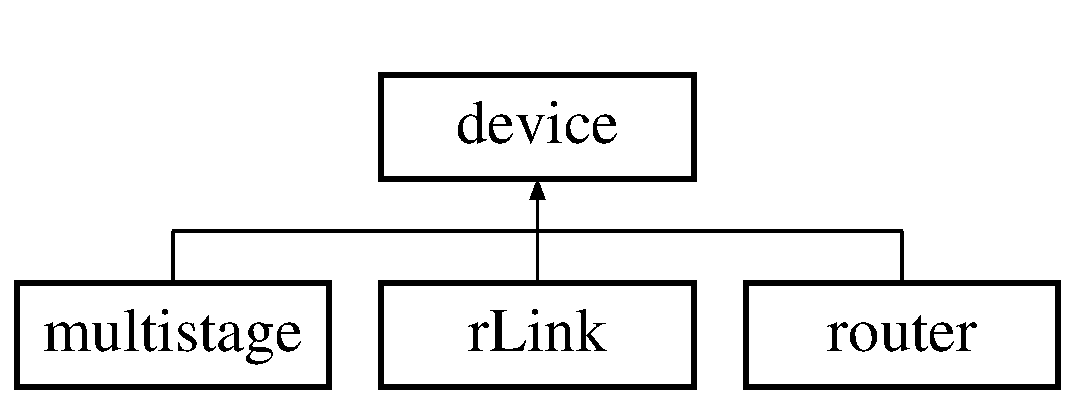
\includegraphics[height=2cm]{classdevice}
\end{center}
\end{figure}
\subsection*{Public Member Functions}
\begin{DoxyCompactItemize}
\item 
\hyperlink{classdevice_a95ab42e0b2e738637d3414347fa5559c}{device} ()
\begin{DoxyCompactList}\small\item\em Construct empty device. \item\end{DoxyCompactList}\item 
\hyperlink{classdevice_a57b9c4ac7a8bd970b81b1154ae79a5de}{device} (int, string, double, double, int, int)
\begin{DoxyCompactList}\small\item\em Construct multistage architecture and routers there in. \item\end{DoxyCompactList}\item 
\hyperlink{classdevice_a3aa4a2a68f49628354dbe33de584f726}{device} (int, string, double, double, int)
\begin{DoxyCompactList}\small\item\em Construct multistage architecture and routers there in. \item\end{DoxyCompactList}\item 
\hyperlink{classdevice_a08545ac77231c68a27c32633a9730a33}{$\sim$device} ()
\begin{DoxyCompactList}\small\item\em destructor \item\end{DoxyCompactList}\item 
int \hyperlink{classdevice_a5b73405bc8184085f92306d4f323b572}{getID} ()
\begin{DoxyCompactList}\small\item\em Gets device identification number. \item\end{DoxyCompactList}\item 
string \hyperlink{classdevice_a9dc7119476febd7ba47060d74ba37e20}{getName} ()
\begin{DoxyCompactList}\small\item\em Gets device name. \item\end{DoxyCompactList}\item 
double \hyperlink{classdevice_ae444f5ce9e539235bc5df36f7b47609c}{getCapacity} ()
\begin{DoxyCompactList}\small\item\em Gets device capacity. \item\end{DoxyCompactList}\item 
double \hyperlink{classdevice_af7b6d78ad457ad75a5f3ed2b40266017}{getPower} ()
\begin{DoxyCompactList}\small\item\em Gets device power consumption. \item\end{DoxyCompactList}\item 
bool \hyperlink{classdevice_a287ef719b436c552cb78f498869ce590}{getState} ()
\begin{DoxyCompactList}\small\item\em Gets device state. \item\end{DoxyCompactList}\item 
int \hyperlink{classdevice_aba1387d01eac1fa58a5386395b368384}{getNr\_\-device} ()
\begin{DoxyCompactList}\small\item\em Gets number of devices contained inside a device. \item\end{DoxyCompactList}\item 
void \hyperlink{classdevice_a66b66e2bce25b091d651ee6336f6f40e}{setCapacity} (double)
\begin{DoxyCompactList}\small\item\em Sets device capacity. \item\end{DoxyCompactList}\item 
void \hyperlink{classdevice_a43b8093ad785d5b5787751a7ede0ae73}{setPower} (double)
\begin{DoxyCompactList}\small\item\em Sets device power consumption. \item\end{DoxyCompactList}\item 
void \hyperlink{classdevice_a8479767364d2d7a6e349552eb6bae023}{setState} (bool)
\begin{DoxyCompactList}\small\item\em Sets device state. \item\end{DoxyCompactList}\end{DoxyCompactItemize}


\subsection{Detailed Description}
Basic class for devices in the multistage architecture. Inherited by multistage, routers and links 

\subsection{Constructor \& Destructor Documentation}
\hypertarget{classdevice_a95ab42e0b2e738637d3414347fa5559c}{
\index{device@{device}!device@{device}}
\index{device@{device}!device@{device}}
\subsubsection[{device}]{\setlength{\rightskip}{0pt plus 5cm}device::device ()\hspace{0.3cm}{\ttfamily  \mbox{[}inline\mbox{]}}}}
\label{classdevice_a95ab42e0b2e738637d3414347fa5559c}


Construct empty device. 

\hypertarget{classdevice_a57b9c4ac7a8bd970b81b1154ae79a5de}{
\index{device@{device}!device@{device}}
\index{device@{device}!device@{device}}
\subsubsection[{device}]{\setlength{\rightskip}{0pt plus 5cm}device::device (int {\em ID}, \/  string {\em name}, \/  double {\em capacity}, \/  double {\em power}, \/  int {\em state}, \/  int {\em nr\_\-device})}}
\label{classdevice_a57b9c4ac7a8bd970b81b1154ae79a5de}


Construct multistage architecture and routers there in. 


\begin{DoxyParams}{Parameters}
\item[{\em ID}]device identification number \item[{\em name}]device name \item[{\em capacity}]device capacity \item[{\em power}]device power consumption \item[{\em nr\_\-device}]number of devices contained inside: multistage contain routers and routers contain links \item[{\em state}]device state: ON/OFF \end{DoxyParams}
\hypertarget{classdevice_a3aa4a2a68f49628354dbe33de584f726}{
\index{device@{device}!device@{device}}
\index{device@{device}!device@{device}}
\subsubsection[{device}]{\setlength{\rightskip}{0pt plus 5cm}device::device (int {\em ID}, \/  string {\em name}, \/  double {\em capacity}, \/  double {\em power}, \/  int {\em state})}}
\label{classdevice_a3aa4a2a68f49628354dbe33de584f726}


Construct multistage architecture and routers there in. 


\begin{DoxyParams}{Parameters}
\item[{\em ID}]device identification \item[{\em name}]device name \item[{\em capacity}]device capacity \item[{\em power}]device power consumption \item[{\em state}]device state: ON/OFF \end{DoxyParams}
\hypertarget{classdevice_a08545ac77231c68a27c32633a9730a33}{
\index{device@{device}!$\sim$device@{$\sim$device}}
\index{$\sim$device@{$\sim$device}!device@{device}}
\subsubsection[{$\sim$device}]{\setlength{\rightskip}{0pt plus 5cm}device::$\sim$device ()\hspace{0.3cm}{\ttfamily  \mbox{[}inline\mbox{]}}}}
\label{classdevice_a08545ac77231c68a27c32633a9730a33}


destructor 



\subsection{Member Function Documentation}
\hypertarget{classdevice_ae444f5ce9e539235bc5df36f7b47609c}{
\index{device@{device}!getCapacity@{getCapacity}}
\index{getCapacity@{getCapacity}!device@{device}}
\subsubsection[{getCapacity}]{\setlength{\rightskip}{0pt plus 5cm}double device::getCapacity ()}}
\label{classdevice_ae444f5ce9e539235bc5df36f7b47609c}


Gets device capacity. 

\begin{DoxyReturn}{Returns}
device capacity 
\end{DoxyReturn}
\hypertarget{classdevice_a5b73405bc8184085f92306d4f323b572}{
\index{device@{device}!getID@{getID}}
\index{getID@{getID}!device@{device}}
\subsubsection[{getID}]{\setlength{\rightskip}{0pt plus 5cm}int device::getID ()}}
\label{classdevice_a5b73405bc8184085f92306d4f323b572}


Gets device identification number. 

\begin{DoxyReturn}{Returns}
device identification number 
\end{DoxyReturn}
\hypertarget{classdevice_a9dc7119476febd7ba47060d74ba37e20}{
\index{device@{device}!getName@{getName}}
\index{getName@{getName}!device@{device}}
\subsubsection[{getName}]{\setlength{\rightskip}{0pt plus 5cm}string device::getName ()}}
\label{classdevice_a9dc7119476febd7ba47060d74ba37e20}


Gets device name. 

\begin{DoxyReturn}{Returns}
device name 
\end{DoxyReturn}
\hypertarget{classdevice_aba1387d01eac1fa58a5386395b368384}{
\index{device@{device}!getNr\_\-device@{getNr\_\-device}}
\index{getNr\_\-device@{getNr\_\-device}!device@{device}}
\subsubsection[{getNr\_\-device}]{\setlength{\rightskip}{0pt plus 5cm}int device::getNr\_\-device ()}}
\label{classdevice_aba1387d01eac1fa58a5386395b368384}


Gets number of devices contained inside a device. 

\begin{DoxyReturn}{Returns}
Number of devices contained inside a device. For example the number of routers in a multistage architecture 
\end{DoxyReturn}
\hypertarget{classdevice_af7b6d78ad457ad75a5f3ed2b40266017}{
\index{device@{device}!getPower@{getPower}}
\index{getPower@{getPower}!device@{device}}
\subsubsection[{getPower}]{\setlength{\rightskip}{0pt plus 5cm}double device::getPower ()}}
\label{classdevice_af7b6d78ad457ad75a5f3ed2b40266017}


Gets device power consumption. 

\begin{DoxyReturn}{Returns}
device power 
\end{DoxyReturn}
\hypertarget{classdevice_a287ef719b436c552cb78f498869ce590}{
\index{device@{device}!getState@{getState}}
\index{getState@{getState}!device@{device}}
\subsubsection[{getState}]{\setlength{\rightskip}{0pt plus 5cm}bool device::getState ()}}
\label{classdevice_a287ef719b436c552cb78f498869ce590}


Gets device state. 

\begin{DoxyReturn}{Returns}
device state 
\end{DoxyReturn}
\hypertarget{classdevice_a66b66e2bce25b091d651ee6336f6f40e}{
\index{device@{device}!setCapacity@{setCapacity}}
\index{setCapacity@{setCapacity}!device@{device}}
\subsubsection[{setCapacity}]{\setlength{\rightskip}{0pt plus 5cm}void device::setCapacity (double {\em capacity})}}
\label{classdevice_a66b66e2bce25b091d651ee6336f6f40e}


Sets device capacity. 


\begin{DoxyParams}{Parameters}
\item[{\em capacity}]capacity of the device \end{DoxyParams}
\hypertarget{classdevice_a43b8093ad785d5b5787751a7ede0ae73}{
\index{device@{device}!setPower@{setPower}}
\index{setPower@{setPower}!device@{device}}
\subsubsection[{setPower}]{\setlength{\rightskip}{0pt plus 5cm}void device::setPower (double {\em power})}}
\label{classdevice_a43b8093ad785d5b5787751a7ede0ae73}


Sets device power consumption. 


\begin{DoxyParams}{Parameters}
\item[{\em power}]power consumption of the device \end{DoxyParams}
\hypertarget{classdevice_a8479767364d2d7a6e349552eb6bae023}{
\index{device@{device}!setState@{setState}}
\index{setState@{setState}!device@{device}}
\subsubsection[{setState}]{\setlength{\rightskip}{0pt plus 5cm}void device::setState (bool {\em state})}}
\label{classdevice_a8479767364d2d7a6e349552eb6bae023}


Sets device state. 


\begin{DoxyParams}{Parameters}
\item[{\em state}]the stare fo the device: ON/OFF \end{DoxyParams}


The documentation for this class was generated from the following files:\begin{DoxyCompactItemize}
\item 
/media/Data/research/code/online\_\-unsplittable\_\-heuristic/include/\hyperlink{device_8h}{device.h}\item 
/media/Data/research/code/online\_\-unsplittable\_\-heuristic/\hyperlink{device_8cpp}{device.cpp}\end{DoxyCompactItemize}

\hypertarget{classdeviceSetup}{
\section{deviceSetup Class Reference}
\label{classdeviceSetup}\index{deviceSetup@{deviceSetup}}
}


sets up the multistage architecture configuration  




{\ttfamily \#include $<$deviceSetup.h$>$}

\subsection*{Public Member Functions}
\begin{DoxyCompactItemize}
\item 
\hyperlink{classdeviceSetup_aee6d5a2f08053ef7071853eaefd4ca42}{deviceSetup} ()
\begin{DoxyCompactList}\small\item\em constructor \item\end{DoxyCompactList}\item 
\hyperlink{classdeviceSetup_a80a771874b29d08f05f92c1b2c52c348}{$\sim$deviceSetup} ()
\begin{DoxyCompactList}\small\item\em destructor \item\end{DoxyCompactList}\item 
void \hyperlink{classdeviceSetup_a56a51cc81222dec1a08e1d07eafca000}{actualCapacity} (\hyperlink{classmultistage}{multistage} $\ast$, list$<$ \hyperlink{classrouter}{router} $>$ \&)
\begin{DoxyCompactList}\small\item\em computes the actual capacity of backend routers \item\end{DoxyCompactList}\item 
void \hyperlink{classdeviceSetup_a89cb8151a7b9153ea09fcfc52260bb9b}{empty\_\-routers} (list$<$ \hyperlink{classrouter}{router} $>$ \&)
\begin{DoxyCompactList}\small\item\em resets some parameters of the router; such as its initial residual capacity \item\end{DoxyCompactList}\item 
void \hyperlink{classdeviceSetup_a5570f97a50fe149a89b9f62500932cec}{part\_\-empty\_\-routers} (list$<$ \hyperlink{classrouter}{router} $>$ \&)
\begin{DoxyCompactList}\small\item\em empty only the router traffic statistics \item\end{DoxyCompactList}\end{DoxyCompactItemize}


\subsection{Detailed Description}
sets up the multistage architecture configuration initially it is needed to initialize the multistage architecture as well as its internal components 

\subsection{Constructor \& Destructor Documentation}
\hypertarget{classdeviceSetup_aee6d5a2f08053ef7071853eaefd4ca42}{
\index{deviceSetup@{deviceSetup}!deviceSetup@{deviceSetup}}
\index{deviceSetup@{deviceSetup}!deviceSetup@{deviceSetup}}
\subsubsection[{deviceSetup}]{\setlength{\rightskip}{0pt plus 5cm}deviceSetup::deviceSetup ()}}
\label{classdeviceSetup_aee6d5a2f08053ef7071853eaefd4ca42}


constructor 

\hypertarget{classdeviceSetup_a80a771874b29d08f05f92c1b2c52c348}{
\index{deviceSetup@{deviceSetup}!$\sim$deviceSetup@{$\sim$deviceSetup}}
\index{$\sim$deviceSetup@{$\sim$deviceSetup}!deviceSetup@{deviceSetup}}
\subsubsection[{$\sim$deviceSetup}]{\setlength{\rightskip}{0pt plus 5cm}deviceSetup::$\sim$deviceSetup ()}}
\label{classdeviceSetup_a80a771874b29d08f05f92c1b2c52c348}


destructor 



\subsection{Member Function Documentation}
\hypertarget{classdeviceSetup_a56a51cc81222dec1a08e1d07eafca000}{
\index{deviceSetup@{deviceSetup}!actualCapacity@{actualCapacity}}
\index{actualCapacity@{actualCapacity}!deviceSetup@{deviceSetup}}
\subsubsection[{actualCapacity}]{\setlength{\rightskip}{0pt plus 5cm}void deviceSetup::actualCapacity ({\bf multistage} $\ast$ {\em mssr}, \/  list$<$ {\bf router} $>$ \& {\em rList})}}
\label{classdeviceSetup_a56a51cc81222dec1a08e1d07eafca000}


computes the actual capacity of backend routers 

the actual capacity of a router is limited either by the total capacity of its links or by its routing capacity 
\begin{DoxyParams}{Parameters}
\item[{\em mssr}]the multistage architecture \item[{\em rList}]the list of routers in the multistage architecture \end{DoxyParams}
\hypertarget{classdeviceSetup_a89cb8151a7b9153ea09fcfc52260bb9b}{
\index{deviceSetup@{deviceSetup}!empty\_\-routers@{empty\_\-routers}}
\index{empty\_\-routers@{empty\_\-routers}!deviceSetup@{deviceSetup}}
\subsubsection[{empty\_\-routers}]{\setlength{\rightskip}{0pt plus 5cm}void deviceSetup::empty\_\-routers (list$<$ {\bf router} $>$ \& {\em rList})}}
\label{classdeviceSetup_a89cb8151a7b9153ea09fcfc52260bb9b}


resets some parameters of the router; such as its initial residual capacity 


\begin{DoxyParams}{Parameters}
\item[{\em rList}]the list of routers in the multistage architecture \end{DoxyParams}
\hypertarget{classdeviceSetup_a5570f97a50fe149a89b9f62500932cec}{
\index{deviceSetup@{deviceSetup}!part\_\-empty\_\-routers@{part\_\-empty\_\-routers}}
\index{part\_\-empty\_\-routers@{part\_\-empty\_\-routers}!deviceSetup@{deviceSetup}}
\subsubsection[{part\_\-empty\_\-routers}]{\setlength{\rightskip}{0pt plus 5cm}void deviceSetup::part\_\-empty\_\-routers (list$<$ {\bf router} $>$ \& {\em rList})}}
\label{classdeviceSetup_a5570f97a50fe149a89b9f62500932cec}


empty only the router traffic statistics 


\begin{DoxyParams}{Parameters}
\item[{\em rList}]the list of routers in the multistage architecture \end{DoxyParams}


The documentation for this class was generated from the following files:\begin{DoxyCompactItemize}
\item 
/media/Data/research/code/online\_\-unsplittable\_\-heuristic/include/\hyperlink{deviceSetup_8h}{deviceSetup.h}\item 
/media/Data/research/code/online\_\-unsplittable\_\-heuristic/\hyperlink{deviceSetup_8cpp}{deviceSetup.cpp}\end{DoxyCompactItemize}

\hypertarget{classmeasurement}{\section{measurement \-Class \-Reference}
\label{classmeasurement}\index{measurement@{measurement}}
}


used to collect input and output information, gather results  




{\ttfamily \#include $<$measurement.\-h$>$}

\subsection*{\-Public \-Member \-Functions}
\begin{DoxyCompactItemize}
\item 
\hyperlink{classmeasurement_a94ea175b4a5eecf4c60af94b7d630ca0}{measurement} ()
\begin{DoxyCompactList}\small\item\em constructor \end{DoxyCompactList}\item 
\hyperlink{classmeasurement_adad6fad962fe7f356188e2d108069ab9}{$\sim$measurement} ()
\begin{DoxyCompactList}\small\item\em destructor \end{DoxyCompactList}\item 
void \hyperlink{classmeasurement_a18541883e2ecd3b899577809bc318987}{set\-Start} ()
\begin{DoxyCompactList}\small\item\em saves the beginning of the simulation run \end{DoxyCompactList}\item 
void \hyperlink{classmeasurement_adfeee2a53faaa6c4de885f274e31e84f}{set\-End} ()
\begin{DoxyCompactList}\small\item\em saves the end of the simulation run \end{DoxyCompactList}\item 
void \hyperlink{classmeasurement_ab92b9dab0ee6ac312170b5536858fc8c}{set\-Time\-Adv\-List} ()
\begin{DoxyCompactList}\small\item\em sets simulation time list \end{DoxyCompactList}\item 
void \hyperlink{classmeasurement_ae5af86c6b09d4bc3bd8f648c371a3f9c}{set\-Mod\-Time} (char $\ast$)
\begin{DoxyCompactList}\small\item\em set file modification time \end{DoxyCompactList}\item 
vector$<$ long $>$ \hyperlink{classmeasurement_a6348d9460718925850e77c02b8adeba8}{get\-Time\-Adv\-List} ()
\begin{DoxyCompactList}\small\item\em gets simulation time list \end{DoxyCompactList}\item 
double \hyperlink{classmeasurement_a0c29e12029b98174f084e9485c67c10c}{get\-Start} ()
\begin{DoxyCompactList}\small\item\em get simulation start time \end{DoxyCompactList}\item 
double \hyperlink{classmeasurement_a48411dc4fa236d3101ae2ab4c09eebb6}{get\-End} ()
\begin{DoxyCompactList}\small\item\em get simulation end time \end{DoxyCompactList}\item 
long \hyperlink{classmeasurement_ac7aa8bcfc7395295031be31558494d76}{get\-Mod\-Time} ()
\begin{DoxyCompactList}\small\item\em gets file modification time \end{DoxyCompactList}\item 
void \hyperlink{classmeasurement_a18838caa4a3b08613e822aeb449d91ba}{result} (list$<$ \hyperlink{classrouter}{router} $>$, \hyperlink{classstatistics}{statistics})
\begin{DoxyCompactList}\small\item\em display different packing statistics \end{DoxyCompactList}\item 
double \hyperlink{classmeasurement_ab734bbbfdfa01be67553368501b32189}{get\-Sum} (vector$<$ double $>$ \&)
\begin{DoxyCompactList}\small\item\em compute summation of a vector of any type \-T \end{DoxyCompactList}\item 
bool \hyperlink{classmeasurement_abd3271afad2207cd5db4de16edbf59a3}{compare\-Vector} (vector$<$ double $>$ \&, vector$<$ double $>$ \&)
\begin{DoxyCompactList}\small\item\em compare two vectors \end{DoxyCompactList}\item 
int \hyperlink{classmeasurement_a4126bd87377bb02f30d9f81f3d36304c}{conf\-\_\-diff} (list$<$ \hyperlink{classrouter}{router} $>$ \&, list$<$ \hyperlink{classrouter}{router} $>$ \&)
\begin{DoxyCompactList}\small\item\em measure the difference, in terms of nr of router, between current load and previous load \end{DoxyCompactList}\item 
void \hyperlink{classmeasurement_a10e7afbdd82e2fed30bd9e7a8725a3bc}{config\-\_\-file} (list$<$ \hyperlink{classrouter}{router} $>$)
\begin{DoxyCompactList}\small\item\em display the input configuration file parsed \end{DoxyCompactList}\end{DoxyCompactItemize}


\subsection{\-Detailed \-Description}
used to collect input and output information, gather results 

\subsection{\-Constructor \& \-Destructor \-Documentation}
\hypertarget{classmeasurement_a94ea175b4a5eecf4c60af94b7d630ca0}{\index{measurement@{measurement}!measurement@{measurement}}
\index{measurement@{measurement}!measurement@{measurement}}
\subsubsection[{measurement}]{\setlength{\rightskip}{0pt plus 5cm}{\bf measurement\-::measurement} (
\begin{DoxyParamCaption}
{}
\end{DoxyParamCaption}
)}}\label{classmeasurement_a94ea175b4a5eecf4c60af94b7d630ca0}


constructor 

\hypertarget{classmeasurement_adad6fad962fe7f356188e2d108069ab9}{\index{measurement@{measurement}!$\sim$measurement@{$\sim$measurement}}
\index{$\sim$measurement@{$\sim$measurement}!measurement@{measurement}}
\subsubsection[{$\sim$measurement}]{\setlength{\rightskip}{0pt plus 5cm}{\bf measurement\-::$\sim$measurement} (
\begin{DoxyParamCaption}
{}
\end{DoxyParamCaption}
)}}\label{classmeasurement_adad6fad962fe7f356188e2d108069ab9}


destructor 



\subsection{\-Member \-Function \-Documentation}
\hypertarget{classmeasurement_abd3271afad2207cd5db4de16edbf59a3}{\index{measurement@{measurement}!compare\-Vector@{compare\-Vector}}
\index{compare\-Vector@{compare\-Vector}!measurement@{measurement}}
\subsubsection[{compare\-Vector}]{\setlength{\rightskip}{0pt plus 5cm}bool {\bf measurement\-::compare\-Vector} (
\begin{DoxyParamCaption}
\item[{vector$<$ double $>$ \&}]{vector1, }
\item[{vector$<$ double $>$ \&}]{vector2}
\end{DoxyParamCaption}
)}}\label{classmeasurement_abd3271afad2207cd5db4de16edbf59a3}


compare two vectors 

take any two vectors of any type and compare them 
\begin{DoxyParams}{\-Parameters}
{\em vector1} & the first vector (the reference) \\
\hline
{\em vector2} & the second vector to be compared to the first vector \\
\hline
\end{DoxyParams}
\hypertarget{classmeasurement_a4126bd87377bb02f30d9f81f3d36304c}{\index{measurement@{measurement}!conf\-\_\-diff@{conf\-\_\-diff}}
\index{conf\-\_\-diff@{conf\-\_\-diff}!measurement@{measurement}}
\subsubsection[{conf\-\_\-diff}]{\setlength{\rightskip}{0pt plus 5cm}int {\bf measurement\-::conf\-\_\-diff} (
\begin{DoxyParamCaption}
\item[{list$<$ {\bf router} $>$ \&}]{r\-List, }
\item[{list$<$ {\bf router} $>$ \&}]{prev\-\_\-r\-List}
\end{DoxyParamCaption}
)}}\label{classmeasurement_a4126bd87377bb02f30d9f81f3d36304c}


measure the difference, in terms of nr of router, between current load and previous load 

this difference is used to compare with the optimal solution 
\begin{DoxyParams}{\-Parameters}
{\em r\-List} & list of back end routers (current configuration) \\
\hline
{\em prev\-\_\-r\-List} & list of back end routers (previous configuration) \\
\hline
\end{DoxyParams}
\begin{DoxyReturn}{\-Returns}
conf\-\_\-change\-\_\-count difference between the two configuration 
\end{DoxyReturn}
\hypertarget{classmeasurement_a10e7afbdd82e2fed30bd9e7a8725a3bc}{\index{measurement@{measurement}!config\-\_\-file@{config\-\_\-file}}
\index{config\-\_\-file@{config\-\_\-file}!measurement@{measurement}}
\subsubsection[{config\-\_\-file}]{\setlength{\rightskip}{0pt plus 5cm}void {\bf measurement\-::config\-\_\-file} (
\begin{DoxyParamCaption}
\item[{list$<$ {\bf router} $>$}]{r\-List}
\end{DoxyParamCaption}
)}}\label{classmeasurement_a10e7afbdd82e2fed30bd9e7a8725a3bc}


display the input configuration file parsed 

it is a check point to verify if the text configuration is parsed correctly or not 
\begin{DoxyParams}{\-Parameters}
{\em r\-List} & list of backend routers \\
\hline
\end{DoxyParams}
\begin{DoxyReturn}{\-Returns}
configuration file 
\end{DoxyReturn}
\hypertarget{classmeasurement_a48411dc4fa236d3101ae2ab4c09eebb6}{\index{measurement@{measurement}!get\-End@{get\-End}}
\index{get\-End@{get\-End}!measurement@{measurement}}
\subsubsection[{get\-End}]{\setlength{\rightskip}{0pt plus 5cm}double {\bf measurement\-::get\-End} (
\begin{DoxyParamCaption}
{}
\end{DoxyParamCaption}
)}}\label{classmeasurement_a48411dc4fa236d3101ae2ab4c09eebb6}


get simulation end time 

\begin{DoxyReturn}{\-Returns}
simulation end time -\/ since epoch time 
\end{DoxyReturn}
\hypertarget{classmeasurement_ac7aa8bcfc7395295031be31558494d76}{\index{measurement@{measurement}!get\-Mod\-Time@{get\-Mod\-Time}}
\index{get\-Mod\-Time@{get\-Mod\-Time}!measurement@{measurement}}
\subsubsection[{get\-Mod\-Time}]{\setlength{\rightskip}{0pt plus 5cm}long {\bf measurement\-::get\-Mod\-Time} (
\begin{DoxyParamCaption}
{}
\end{DoxyParamCaption}
)}}\label{classmeasurement_ac7aa8bcfc7395295031be31558494d76}


gets file modification time 

\begin{DoxyReturn}{\-Returns}
modification time 
\end{DoxyReturn}
\hypertarget{classmeasurement_a0c29e12029b98174f084e9485c67c10c}{\index{measurement@{measurement}!get\-Start@{get\-Start}}
\index{get\-Start@{get\-Start}!measurement@{measurement}}
\subsubsection[{get\-Start}]{\setlength{\rightskip}{0pt plus 5cm}double {\bf measurement\-::get\-Start} (
\begin{DoxyParamCaption}
{}
\end{DoxyParamCaption}
)}}\label{classmeasurement_a0c29e12029b98174f084e9485c67c10c}


get simulation start time 

\begin{DoxyReturn}{\-Returns}
simulation start time -\/ since epoch time 
\end{DoxyReturn}
\hypertarget{classmeasurement_ab734bbbfdfa01be67553368501b32189}{\index{measurement@{measurement}!get\-Sum@{get\-Sum}}
\index{get\-Sum@{get\-Sum}!measurement@{measurement}}
\subsubsection[{get\-Sum}]{\setlength{\rightskip}{0pt plus 5cm}double {\bf measurement\-::get\-Sum} (
\begin{DoxyParamCaption}
\item[{vector$<$ double $>$ \&}]{vectorin}
\end{DoxyParamCaption}
)}}\label{classmeasurement_ab734bbbfdfa01be67553368501b32189}


compute summation of a vector of any type \-T 


\begin{DoxyParams}{\-Parameters}
{\em vectorin} & \\
\hline
\end{DoxyParams}
\begin{DoxyReturn}{\-Returns}
sum of an input vector 
\end{DoxyReturn}
\hypertarget{classmeasurement_a6348d9460718925850e77c02b8adeba8}{\index{measurement@{measurement}!get\-Time\-Adv\-List@{get\-Time\-Adv\-List}}
\index{get\-Time\-Adv\-List@{get\-Time\-Adv\-List}!measurement@{measurement}}
\subsubsection[{get\-Time\-Adv\-List}]{\setlength{\rightskip}{0pt plus 5cm}vector$<$ long $>$ {\bf measurement\-::get\-Time\-Adv\-List} (
\begin{DoxyParamCaption}
{}
\end{DoxyParamCaption}
)}}\label{classmeasurement_a6348d9460718925850e77c02b8adeba8}


gets simulation time list 

\hypertarget{classmeasurement_a18838caa4a3b08613e822aeb449d91ba}{\index{measurement@{measurement}!result@{result}}
\index{result@{result}!measurement@{measurement}}
\subsubsection[{result}]{\setlength{\rightskip}{0pt plus 5cm}void {\bf measurement\-::result} (
\begin{DoxyParamCaption}
\item[{list$<$ {\bf router} $>$}]{r\-List, }
\item[{{\bf statistics}}]{stat}
\end{DoxyParamCaption}
)}}\label{classmeasurement_a18838caa4a3b08613e822aeb449d91ba}


display different packing statistics 

the statistics dispalyed include simulation time, objective, traffic forwarded and lost, etc 
\begin{DoxyParams}{\-Parameters}
{\em r\-List} & list of backend routers \\
\hline
{\em stat} & statistics about the packing \\
\hline
\end{DoxyParams}
\hypertarget{classmeasurement_adfeee2a53faaa6c4de885f274e31e84f}{\index{measurement@{measurement}!set\-End@{set\-End}}
\index{set\-End@{set\-End}!measurement@{measurement}}
\subsubsection[{set\-End}]{\setlength{\rightskip}{0pt plus 5cm}void {\bf measurement\-::set\-End} (
\begin{DoxyParamCaption}
{}
\end{DoxyParamCaption}
)}}\label{classmeasurement_adfeee2a53faaa6c4de885f274e31e84f}


saves the end of the simulation run 

\hypertarget{classmeasurement_ae5af86c6b09d4bc3bd8f648c371a3f9c}{\index{measurement@{measurement}!set\-Mod\-Time@{set\-Mod\-Time}}
\index{set\-Mod\-Time@{set\-Mod\-Time}!measurement@{measurement}}
\subsubsection[{set\-Mod\-Time}]{\setlength{\rightskip}{0pt plus 5cm}void {\bf measurement\-::set\-Mod\-Time} (
\begin{DoxyParamCaption}
\item[{char $\ast$}]{f\-\_\-name}
\end{DoxyParamCaption}
)}}\label{classmeasurement_ae5af86c6b09d4bc3bd8f648c371a3f9c}


set file modification time 


\begin{DoxyParams}{\-Parameters}
{\em f\-\_\-name} & file name \\
\hline
\end{DoxyParams}
\hypertarget{classmeasurement_a18541883e2ecd3b899577809bc318987}{\index{measurement@{measurement}!set\-Start@{set\-Start}}
\index{set\-Start@{set\-Start}!measurement@{measurement}}
\subsubsection[{set\-Start}]{\setlength{\rightskip}{0pt plus 5cm}void {\bf measurement\-::set\-Start} (
\begin{DoxyParamCaption}
{}
\end{DoxyParamCaption}
)}}\label{classmeasurement_a18541883e2ecd3b899577809bc318987}


saves the beginning of the simulation run 

\hypertarget{classmeasurement_ab92b9dab0ee6ac312170b5536858fc8c}{\index{measurement@{measurement}!set\-Time\-Adv\-List@{set\-Time\-Adv\-List}}
\index{set\-Time\-Adv\-List@{set\-Time\-Adv\-List}!measurement@{measurement}}
\subsubsection[{set\-Time\-Adv\-List}]{\setlength{\rightskip}{0pt plus 5cm}void {\bf measurement\-::set\-Time\-Adv\-List} (
\begin{DoxyParamCaption}
{}
\end{DoxyParamCaption}
)}}\label{classmeasurement_ab92b9dab0ee6ac312170b5536858fc8c}


sets simulation time list 



\-The documentation for this class was generated from the following files\-:\begin{DoxyCompactItemize}
\item 
/media/\-Data/research/code/online\-\_\-unsplittable\-\_\-heuristic/include/\hyperlink{measurement_8h}{measurement.\-h}\item 
/media/\-Data/research/code/online\-\_\-unsplittable\-\_\-heuristic/\hyperlink{measurement_8cpp}{measurement.\-cpp}\end{DoxyCompactItemize}

\hypertarget{classmultistage}{\section{multistage \-Class \-Reference}
\label{classmultistage}\index{multistage@{multistage}}
}


\-Multistage architecture class reference.  




{\ttfamily \#include $<$multistage.\-h$>$}

\-Inheritance diagram for multistage\-:\begin{figure}[H]
\begin{center}
\leavevmode
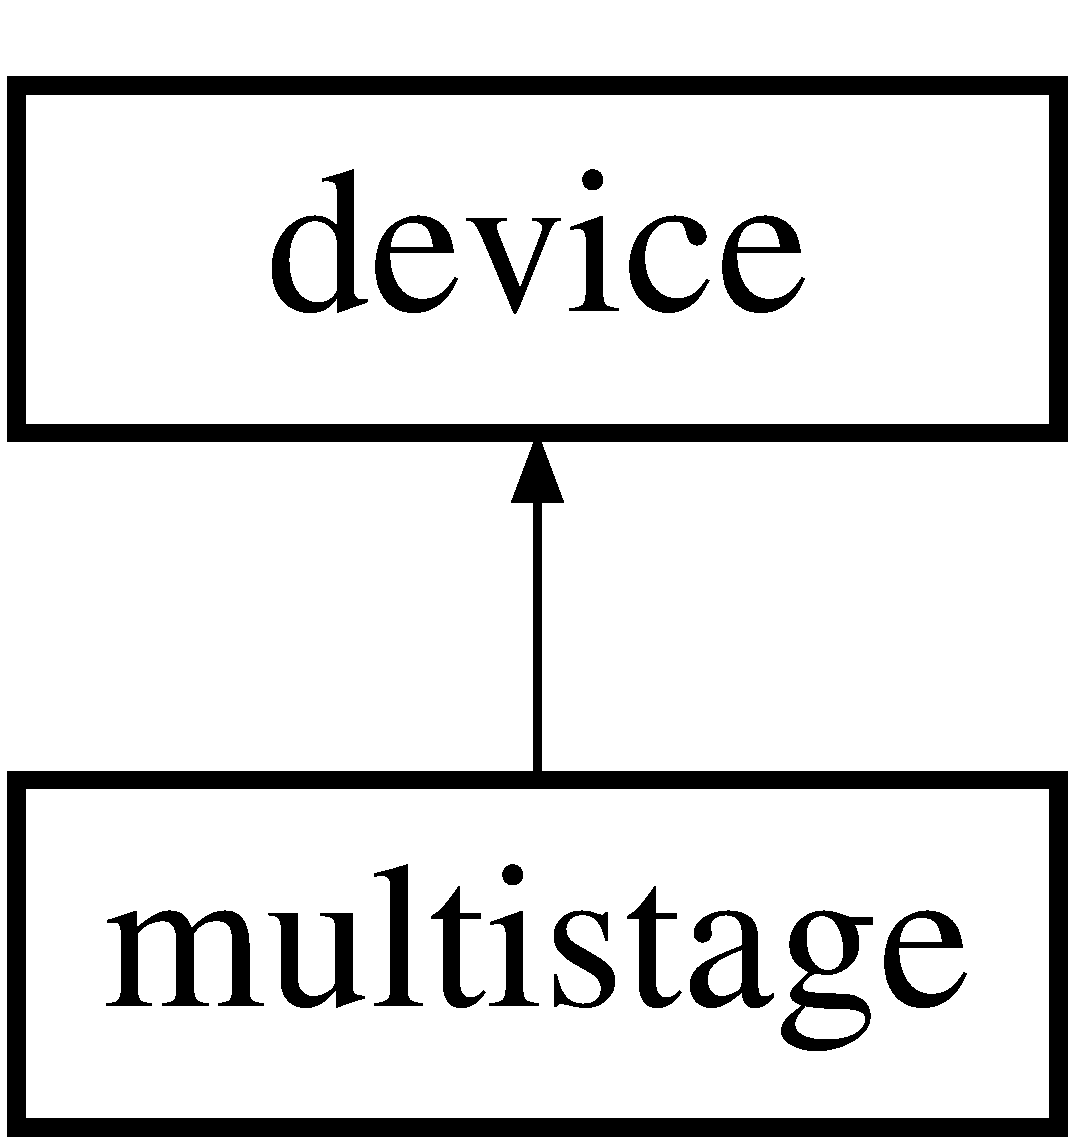
\includegraphics[height=2.000000cm]{classmultistage}
\end{center}
\end{figure}
\subsection*{\-Public \-Member \-Functions}
\begin{DoxyCompactItemize}
\item 
\hyperlink{classmultistage_abbfa555a8fbdfe7f70efa06fddbaa335}{multistage} ()
\begin{DoxyCompactList}\small\item\em constructor \end{DoxyCompactList}\item 
\hyperlink{classmultistage_a3ce104e1cd528efc9f4f2b8b8c2f54a7}{$\sim$multistage} ()
\begin{DoxyCompactList}\small\item\em \-Destructor. \end{DoxyCompactList}\item 
\hyperlink{classmultistage_adcbb45a38e0184f037cdc03504dced05}{multistage} (int, string, double, double, int, int)
\begin{DoxyCompactList}\small\item\em \-Construct a router. \end{DoxyCompactList}\item 
list$<$ \hyperlink{classrouter}{router} $>$ \hyperlink{classmultistage_ad42d7006ba661c60eb4958f8534ad89a}{get\-R\-List} ()
\begin{DoxyCompactList}\small\item\em \-Gets list of routers in an architecture. \end{DoxyCompactList}\item 
void \hyperlink{classmultistage_a6f79ee151acaff9a49e06a3300371a2c}{set\-R\-List} (\hyperlink{classrouter}{router})
\begin{DoxyCompactList}\small\item\em \-Sets an architecture's router list. \end{DoxyCompactList}\end{DoxyCompactItemize}


\subsection{\-Detailed \-Description}
\-Multistage architecture class reference. 

\-It inherits device class and creates a new multistage architecture with list of routers and sets total architecture actual capacity.

{\bfseries \-Usage \-Example\-:} 
\begin{DoxyCode}
 multistage *m = new multistage(1, "mssr", 0, 0, 0, 0)
\end{DoxyCode}
 \begin{DoxySeeAlso}{\-See also}
\hyperlink{classdevice_a57b9c4ac7a8bd970b81b1154ae79a5de}{device(int ,string ,double ,double ,int ,int )} 
\end{DoxySeeAlso}


\subsection{\-Constructor \& \-Destructor \-Documentation}
\hypertarget{classmultistage_abbfa555a8fbdfe7f70efa06fddbaa335}{\index{multistage@{multistage}!multistage@{multistage}}
\index{multistage@{multistage}!multistage@{multistage}}
\subsubsection[{multistage}]{\setlength{\rightskip}{0pt plus 5cm}{\bf multistage\-::multistage} (
\begin{DoxyParamCaption}
{}
\end{DoxyParamCaption}
)}}\label{classmultistage_abbfa555a8fbdfe7f70efa06fddbaa335}


constructor 

\hypertarget{classmultistage_a3ce104e1cd528efc9f4f2b8b8c2f54a7}{\index{multistage@{multistage}!$\sim$multistage@{$\sim$multistage}}
\index{$\sim$multistage@{$\sim$multistage}!multistage@{multistage}}
\subsubsection[{$\sim$multistage}]{\setlength{\rightskip}{0pt plus 5cm}{\bf multistage\-::$\sim$multistage} (
\begin{DoxyParamCaption}
{}
\end{DoxyParamCaption}
)}}\label{classmultistage_a3ce104e1cd528efc9f4f2b8b8c2f54a7}


\-Destructor. 

\hypertarget{classmultistage_adcbb45a38e0184f037cdc03504dced05}{\index{multistage@{multistage}!multistage@{multistage}}
\index{multistage@{multistage}!multistage@{multistage}}
\subsubsection[{multistage}]{\setlength{\rightskip}{0pt plus 5cm}{\bf multistage\-::multistage} (
\begin{DoxyParamCaption}
\item[{int}]{\-I\-D, }
\item[{string}]{name, }
\item[{double}]{capacity, }
\item[{double}]{power, }
\item[{int}]{state, }
\item[{int}]{nr\-\_\-routers}
\end{DoxyParamCaption}
)}}\label{classmultistage_adcbb45a38e0184f037cdc03504dced05}


\-Construct a router. 


\begin{DoxyParams}{\-Parameters}
{\em \-I\-D} & multistage architecture identification number \\
\hline
{\em name} & multistage architecture name \\
\hline
{\em capacity} & multistage architecture capacity \\
\hline
{\em power} & multistage architecture power consumption \\
\hline
{\em nr\-\_\-routers} & number of routers contained inside a multistage architecture \\
\hline
{\em state} & a multistage architecture state\-: \-O\-N/\-O\-F\-F \\
\hline
\end{DoxyParams}
\begin{DoxySeeAlso}{\-See also}
\hyperlink{classdevice_a57b9c4ac7a8bd970b81b1154ae79a5de}{device(int ,string ,double ,double ,int ,int )} 
\end{DoxySeeAlso}


\subsection{\-Member \-Function \-Documentation}
\hypertarget{classmultistage_ad42d7006ba661c60eb4958f8534ad89a}{\index{multistage@{multistage}!get\-R\-List@{get\-R\-List}}
\index{get\-R\-List@{get\-R\-List}!multistage@{multistage}}
\subsubsection[{get\-R\-List}]{\setlength{\rightskip}{0pt plus 5cm}list$<$ {\bf router} $>$ {\bf multistage\-::get\-R\-List} (
\begin{DoxyParamCaption}
{}
\end{DoxyParamCaption}
)}}\label{classmultistage_ad42d7006ba661c60eb4958f8534ad89a}


\-Gets list of routers in an architecture. 

\begin{DoxyReturn}{\-Returns}
a multistage architecture's router list 
\end{DoxyReturn}
\hypertarget{classmultistage_a6f79ee151acaff9a49e06a3300371a2c}{\index{multistage@{multistage}!set\-R\-List@{set\-R\-List}}
\index{set\-R\-List@{set\-R\-List}!multistage@{multistage}}
\subsubsection[{set\-R\-List}]{\setlength{\rightskip}{0pt plus 5cm}void {\bf multistage\-::set\-R\-List} (
\begin{DoxyParamCaption}
\item[{{\bf router}}]{r}
\end{DoxyParamCaption}
)}}\label{classmultistage_a6f79ee151acaff9a49e06a3300371a2c}


\-Sets an architecture's router list. 


\begin{DoxyParams}{\-Parameters}
{\em r} & router with all its attributes \\
\hline
\end{DoxyParams}


\-The documentation for this class was generated from the following files\-:\begin{DoxyCompactItemize}
\item 
/media/\-Data/research/code/online\-\_\-unsplittable\-\_\-heuristic/include/\hyperlink{multistage_8h}{multistage.\-h}\item 
/media/\-Data/research/code/online\-\_\-unsplittable\-\_\-heuristic/\hyperlink{multistage_8cpp}{multistage.\-cpp}\end{DoxyCompactItemize}

\hypertarget{classpacking}{
\section{packing Class Reference}
\label{classpacking}\index{packing@{packing}}
}


Implementation of bin packing algorithms.  




{\ttfamily \#include $<$packing.h$>$}

\subsection*{Public Member Functions}
\begin{DoxyCompactItemize}
\item 
\hyperlink{classpacking_ad0cae9459a9abfe4bf76642a232ec2f3}{packing} ()
\begin{DoxyCompactList}\small\item\em default constructor \item\end{DoxyCompactList}\item 
\hyperlink{classpacking_a985cd1712c1e0c7e9f3927e847383810}{$\sim$packing} ()
\begin{DoxyCompactList}\small\item\em default destructor \item\end{DoxyCompactList}\item 
\hyperlink{classstatistics}{statistics} \hyperlink{classpacking_aa80d123e13482fc9760fd87e44f27e0f}{bin\_\-packing} (vector$<$ double $>$ \&, list$<$ \hyperlink{classrouter}{router} $>$ \&)
\begin{DoxyCompactList}\small\item\em Interface to packing algorithms. \item\end{DoxyCompactList}\item 
void \hyperlink{classpacking_acd308605e21d05122f19b6673f7496a2}{ff} (vector$<$ double $>$ \&, list$<$ \hyperlink{classrouter}{router} $>$ \&)
\begin{DoxyCompactList}\small\item\em First Fit bin packing algorithm. \item\end{DoxyCompactList}\end{DoxyCompactItemize}


\subsection{Detailed Description}
Implementation of bin packing algorithms. REFERENCE: Approximation algorithms for bin packing: A survey
\begin{DoxyItemize}
\item First fit (ff) -\/ implemented
\item First fit decreasing (ffd) -\/ implemented
\item Best fit (bf) -\/ not yet implemented
\item Best fit decreasing (bfd) -\/ not yet implemented
\item Worst fit (wf) -\/ not yet implemented
\item Worst fir decreasing (wfd) -\/ not yet implemented 
\end{DoxyItemize}

\subsection{Constructor \& Destructor Documentation}
\hypertarget{classpacking_ad0cae9459a9abfe4bf76642a232ec2f3}{
\index{packing@{packing}!packing@{packing}}
\index{packing@{packing}!packing@{packing}}
\subsubsection[{packing}]{\setlength{\rightskip}{0pt plus 5cm}packing::packing ()}}
\label{classpacking_ad0cae9459a9abfe4bf76642a232ec2f3}


default constructor 

\hypertarget{classpacking_a985cd1712c1e0c7e9f3927e847383810}{
\index{packing@{packing}!$\sim$packing@{$\sim$packing}}
\index{$\sim$packing@{$\sim$packing}!packing@{packing}}
\subsubsection[{$\sim$packing}]{\setlength{\rightskip}{0pt plus 5cm}packing::$\sim$packing ()}}
\label{classpacking_a985cd1712c1e0c7e9f3927e847383810}


default destructor 



\subsection{Member Function Documentation}
\hypertarget{classpacking_aa80d123e13482fc9760fd87e44f27e0f}{
\index{packing@{packing}!bin\_\-packing@{bin\_\-packing}}
\index{bin\_\-packing@{bin\_\-packing}!packing@{packing}}
\subsubsection[{bin\_\-packing}]{\setlength{\rightskip}{0pt plus 5cm}{\bf statistics} packing::bin\_\-packing (vector$<$ double $>$ \& {\em trafficToPack}, \/  list$<$ {\bf router} $>$ \& {\em r\_\-list})}}
\label{classpacking_aa80d123e13482fc9760fd87e44f27e0f}


Interface to packing algorithms. 


\begin{DoxyParams}{Parameters}
\item[{\em trafficToPack}]input traffic for packing \item[{\em r\_\-list}]list of routers to pack \end{DoxyParams}
\begin{DoxyReturn}{Returns}
packing statistics 
\end{DoxyReturn}
\hypertarget{classpacking_acd308605e21d05122f19b6673f7496a2}{
\index{packing@{packing}!ff@{ff}}
\index{ff@{ff}!packing@{packing}}
\subsubsection[{ff}]{\setlength{\rightskip}{0pt plus 5cm}void packing::ff (vector$<$ double $>$ \& {\em trafficToPack}, \/  list$<$ {\bf router} $>$ \& {\em r\_\-list})}}
\label{classpacking_acd308605e21d05122f19b6673f7496a2}


First Fit bin packing algorithm. 

forward a flow using the first available backend router and the first available link on that router which have a capacity to handle the flow. If such a router is not available, drop the flow. 
\begin{DoxyParams}{Parameters}
\item[{\em trafficToPack}]input traffic for packing \item[{\em r\_\-list}]list of routers to pack \end{DoxyParams}
\begin{DoxyReturn}{Returns}
r\_\-list list of routers PROCESS:
\begin{DoxyItemize}
\item forward a flow using the first available router and the first link available on that router that can handle the flow
\item update different flow statistics such as residual capacity of a currently used link, lost flows, objective value, etc., on the way 
\end{DoxyItemize}
\end{DoxyReturn}


if flow fits into a link, compute the residual capacity of both the router and the link 



The documentation for this class was generated from the following files:\begin{DoxyCompactItemize}
\item 
/media/Data/research/code/online\_\-unsplittable\_\-heuristic/include/\hyperlink{packing_8h}{packing.h}\item 
/media/Data/research/code/online\_\-unsplittable\_\-heuristic/\hyperlink{packing_8cpp}{packing.cpp}\end{DoxyCompactItemize}

\hypertarget{classparser}{
\section{parser Class Reference}
\label{classparser}\index{parser@{parser}}
}


parse command line parameters and input configuration file  




{\ttfamily \#include $<$parser.h$>$}

\subsection*{Public Member Functions}
\begin{DoxyCompactItemize}
\item 
\hyperlink{classparser_ac4cb16e924a735dfb5837772afa1a1a9}{parser} ()
\begin{DoxyCompactList}\small\item\em constructor \item\end{DoxyCompactList}\item 
\hyperlink{classparser_acdd4eb1b51b876954c2f7605f65388ce}{$\sim$parser} ()
\begin{DoxyCompactList}\small\item\em destructor \item\end{DoxyCompactList}\item 
void \hyperlink{classparser_ac578bbb7b49c579bc4520a806fb316c5}{cmd\_\-parser} (int, char $\ast$$\ast$)
\begin{DoxyCompactList}\small\item\em parse command line arguments \item\end{DoxyCompactList}\item 
void \hyperlink{classparser_a4bcf9f11cfbb793a414221fafd4c4a7d}{input\_\-parser} (string)
\begin{DoxyCompactList}\small\item\em parse backend router parameters from CPLEX\_\-OPL configuration file \item\end{DoxyCompactList}\item 
void \hyperlink{classparser_a30a37d82f9894b3c725e2dd1daa0234f}{input\_\-traffic} (string)
\begin{DoxyCompactList}\small\item\em parse input traffic \item\end{DoxyCompactList}\item 
void \hyperlink{classparser_a6e2620bd81e91a69dc479f307c8b8b72}{usage} (const char $\ast$, int)
\begin{DoxyCompactList}\small\item\em parse the command line. \item\end{DoxyCompactList}\item 
bool \hyperlink{classparser_a8afa4de9b61d1d11a85de1c00041e69b}{isOdd} (int)
\begin{DoxyCompactList}\small\item\em check if an integer value is odd or not \item\end{DoxyCompactList}\end{DoxyCompactItemize}


\subsection{Detailed Description}
parse command line parameters and input configuration file 

\subsection{Constructor \& Destructor Documentation}
\hypertarget{classparser_ac4cb16e924a735dfb5837772afa1a1a9}{
\index{parser@{parser}!parser@{parser}}
\index{parser@{parser}!parser@{parser}}
\subsubsection[{parser}]{\setlength{\rightskip}{0pt plus 5cm}parser::parser ()}}
\label{classparser_ac4cb16e924a735dfb5837772afa1a1a9}


constructor 

\hypertarget{classparser_acdd4eb1b51b876954c2f7605f65388ce}{
\index{parser@{parser}!$\sim$parser@{$\sim$parser}}
\index{$\sim$parser@{$\sim$parser}!parser@{parser}}
\subsubsection[{$\sim$parser}]{\setlength{\rightskip}{0pt plus 5cm}parser::$\sim$parser ()}}
\label{classparser_acdd4eb1b51b876954c2f7605f65388ce}


destructor 



\subsection{Member Function Documentation}
\hypertarget{classparser_ac578bbb7b49c579bc4520a806fb316c5}{
\index{parser@{parser}!cmd\_\-parser@{cmd\_\-parser}}
\index{cmd\_\-parser@{cmd\_\-parser}!parser@{parser}}
\subsubsection[{cmd\_\-parser}]{\setlength{\rightskip}{0pt plus 5cm}void parser::cmd\_\-parser (int {\em argc}, \/  char $\ast$$\ast$ {\em argv})}}
\label{classparser_ac578bbb7b49c579bc4520a806fb316c5}


parse command line arguments 

input parameters for the simulation are taken from command line. 
\begin{DoxyParams}{Parameters}
\item[{\em argc}]number of input arguments \item[{\em argv}]input arguments \end{DoxyParams}
\hypertarget{classparser_a4bcf9f11cfbb793a414221fafd4c4a7d}{
\index{parser@{parser}!input\_\-parser@{input\_\-parser}}
\index{input\_\-parser@{input\_\-parser}!parser@{parser}}
\subsubsection[{input\_\-parser}]{\setlength{\rightskip}{0pt plus 5cm}void parser::input\_\-parser (string {\em config\_\-file})}}
\label{classparser_a4bcf9f11cfbb793a414221fafd4c4a7d}


parse backend router parameters from CPLEX\_\-OPL configuration file 

different internal components parameters are read from a text input file 
\begin{DoxyParams}{Parameters}
\item[{\em config\_\-file}]CPLEX\_\-OPL formate configuration file \end{DoxyParams}
\begin{DoxyReturn}{Returns}
traffic input traffic 

r\_\-list list of routers class 
\end{DoxyReturn}
\hypertarget{classparser_a30a37d82f9894b3c725e2dd1daa0234f}{
\index{parser@{parser}!input\_\-traffic@{input\_\-traffic}}
\index{input\_\-traffic@{input\_\-traffic}!parser@{parser}}
\subsubsection[{input\_\-traffic}]{\setlength{\rightskip}{0pt plus 5cm}void parser::input\_\-traffic (string {\em config\_\-file})}}
\label{classparser_a30a37d82f9894b3c725e2dd1daa0234f}


parse input traffic 

this function is dedicated to get the traffic line from the configuration file and convert it into a traffic vector 
\begin{DoxyParams}{Parameters}
\item[{\em config\_\-file}]the name of the configuration file \end{DoxyParams}
\hypertarget{classparser_a8afa4de9b61d1d11a85de1c00041e69b}{
\index{parser@{parser}!isOdd@{isOdd}}
\index{isOdd@{isOdd}!parser@{parser}}
\subsubsection[{isOdd}]{\setlength{\rightskip}{0pt plus 5cm}bool parser::isOdd (int {\em count})\hspace{0.3cm}{\ttfamily  \mbox{[}inline\mbox{]}}}}
\label{classparser_a8afa4de9b61d1d11a85de1c00041e69b}


check if an integer value is odd or not 

\hypertarget{classparser_a6e2620bd81e91a69dc479f307c8b8b72}{
\index{parser@{parser}!usage@{usage}}
\index{usage@{usage}!parser@{parser}}
\subsubsection[{usage}]{\setlength{\rightskip}{0pt plus 5cm}void parser::usage (const char $\ast$ {\em program\_\-name}, \/  int {\em exit\_\-code})\hspace{0.3cm}{\ttfamily  \mbox{[}inline\mbox{]}}}}
\label{classparser_a6e2620bd81e91a69dc479f307c8b8b72}


parse the command line. 

command line usage information


\begin{DoxyParams}{Parameters}
\item[{\em program\_\-name}]the name of the executable \item[{\em exit\_\-code}]if the programs exits without execution, indicate why it is not \end{DoxyParams}


The documentation for this class was generated from the following files:\begin{DoxyCompactItemize}
\item 
/media/Data/research/code/online\_\-unsplittable\_\-heuristic/include/\hyperlink{parser_8h}{parser.h}\item 
/media/Data/research/code/online\_\-unsplittable\_\-heuristic/\hyperlink{parser_8cpp}{parser.cpp}\end{DoxyCompactItemize}

\hypertarget{classrLink}{
\section{rLink Class Reference}
\label{classrLink}\index{rLink@{rLink}}
}


Router link class reference.  




{\ttfamily \#include $<$rLink.h$>$}

Inheritance diagram for rLink:\begin{figure}[H]
\begin{center}
\leavevmode
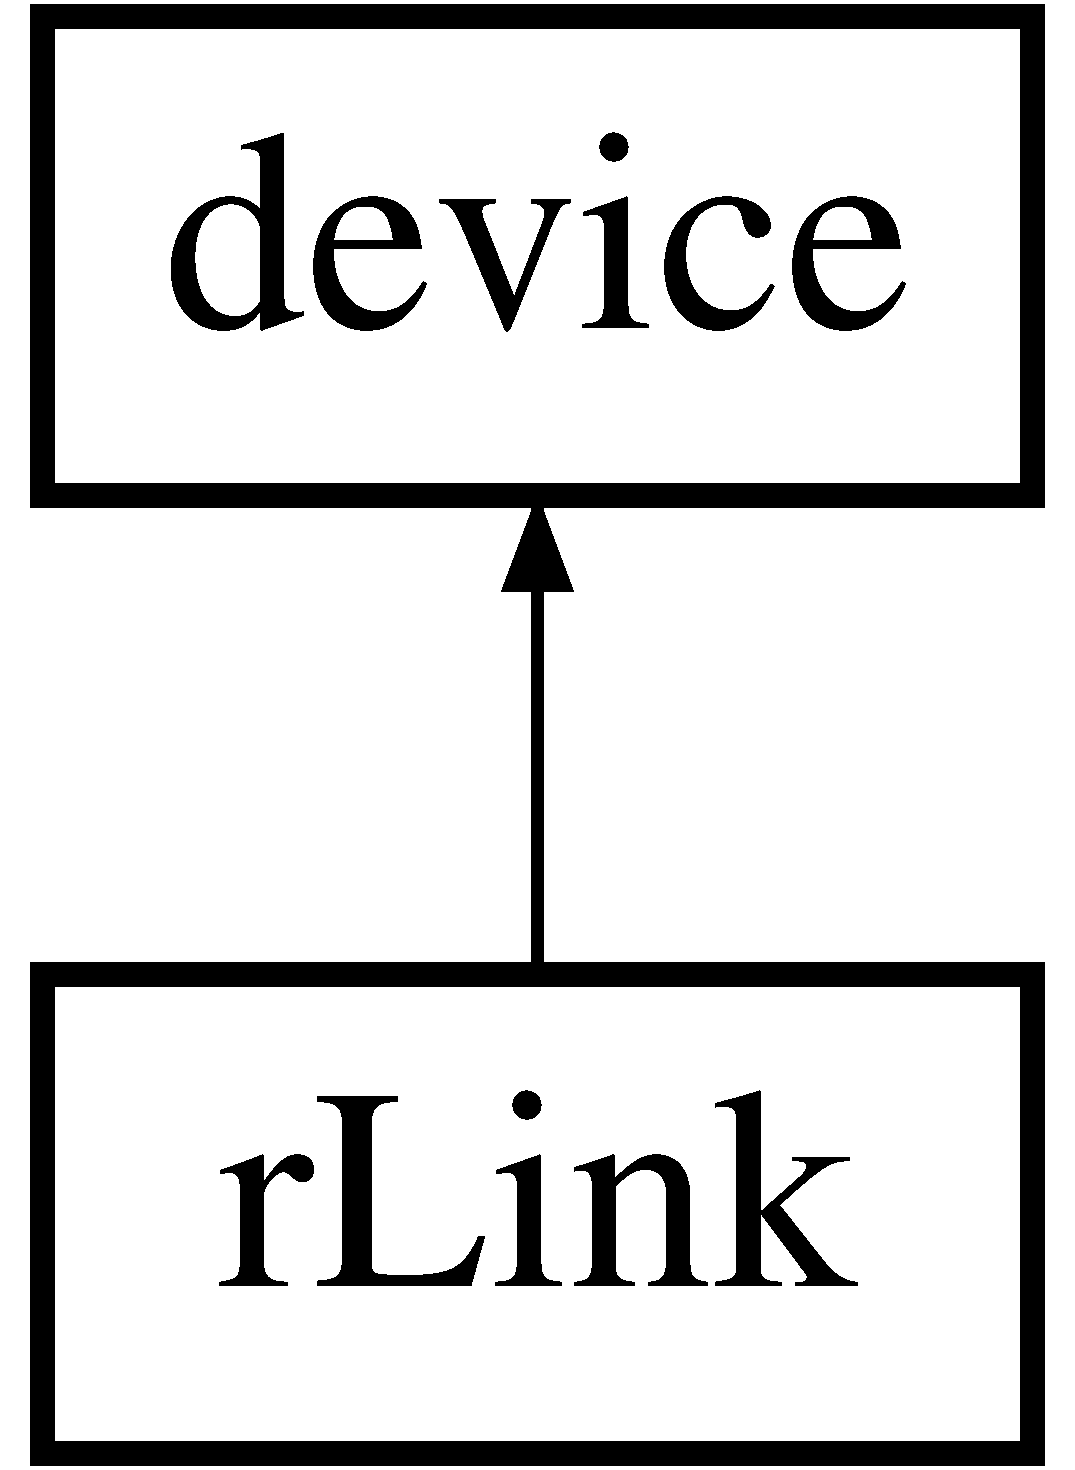
\includegraphics[height=2cm]{classrLink}
\end{center}
\end{figure}
\subsection*{Public Member Functions}
\begin{DoxyCompactItemize}
\item 
\hyperlink{classrLink_acd7f5f66409693e86cd33e4a6e6964b8}{rLink} (int, string, double, double, int)
\begin{DoxyCompactList}\small\item\em Construct a link. \item\end{DoxyCompactList}\item 
\hyperlink{classrLink_ac2f6e30278ba2967b96086435711f672}{$\sim$rLink} ()
\begin{DoxyCompactList}\small\item\em Destructor. \item\end{DoxyCompactList}\item 
double \hyperlink{classrLink_aa840b5668425c224a451ec1663754a82}{getResidual} ()
\begin{DoxyCompactList}\small\item\em Gets residual capacity of a link. \item\end{DoxyCompactList}\item 
bool \hyperlink{classrLink_a4639d6b69acbb669d0cbb7af5cbf152b}{getFlag} ()
\begin{DoxyCompactList}\small\item\em Gets link usage flag. \item\end{DoxyCompactList}\item 
vector$<$ double $>$ \hyperlink{classrLink_a86c80f0a22f7703601d8a242c2fb471f}{getLstat} ()
\begin{DoxyCompactList}\small\item\em Gets link flow statistics. \item\end{DoxyCompactList}\item 
void \hyperlink{classrLink_a7ac5fdbd1b4fc92cbfd5d8e421477148}{setResidual} (double)
\begin{DoxyCompactList}\small\item\em Sets residual capacity of a link. \item\end{DoxyCompactList}\item 
void \hyperlink{classrLink_a15022659ea92d086138f817203ede689}{setFlag} (bool)
\begin{DoxyCompactList}\small\item\em Sets link flag. \item\end{DoxyCompactList}\item 
void \hyperlink{classrLink_a719c8cee2887f566dd4e0ca6df81f0de}{setLstat} (double)
\begin{DoxyCompactList}\small\item\em Sets link flow statistics. \item\end{DoxyCompactList}\item 
void \hyperlink{classrLink_a60204cffa46245fb1e2c7d7a7872dbcb}{clearLstat} ()
\begin{DoxyCompactList}\small\item\em clear link flow statistics \item\end{DoxyCompactList}\end{DoxyCompactItemize}


\subsection{Detailed Description}
Router link class reference. It inherits device class and creates a new link

{\bfseries Usage Example:} 
\begin{DoxyCode}
 rLink *l = new rLink(1, "link_1", 0, 0, 0, 0)
\end{DoxyCode}
 

\subsection{Constructor \& Destructor Documentation}
\hypertarget{classrLink_acd7f5f66409693e86cd33e4a6e6964b8}{
\index{rLink@{rLink}!rLink@{rLink}}
\index{rLink@{rLink}!rLink@{rLink}}
\subsubsection[{rLink}]{\setlength{\rightskip}{0pt plus 5cm}rLink::rLink (int {\em ID}, \/  string {\em name}, \/  double {\em capacity}, \/  double {\em power}, \/  int {\em state})}}
\label{classrLink_acd7f5f66409693e86cd33e4a6e6964b8}


Construct a link. 


\begin{DoxyParams}{Parameters}
\item[{\em ID}]link identification number \item[{\em name}]link name \item[{\em capacity}]link capacity \item[{\em power}]link power consumption \item[{\em state}]link state: ON/OFF \end{DoxyParams}
\begin{DoxySeeAlso}{See also}
\hyperlink{classdevice_a57b9c4ac7a8bd970b81b1154ae79a5de}{device(int ,string ,double ,double ,int ,int )} 
\end{DoxySeeAlso}
\hypertarget{classrLink_ac2f6e30278ba2967b96086435711f672}{
\index{rLink@{rLink}!$\sim$rLink@{$\sim$rLink}}
\index{$\sim$rLink@{$\sim$rLink}!rLink@{rLink}}
\subsubsection[{$\sim$rLink}]{\setlength{\rightskip}{0pt plus 5cm}rLink::$\sim$rLink ()\hspace{0.3cm}{\ttfamily  \mbox{[}inline\mbox{]}}}}
\label{classrLink_ac2f6e30278ba2967b96086435711f672}


Destructor. 



\subsection{Member Function Documentation}
\hypertarget{classrLink_a60204cffa46245fb1e2c7d7a7872dbcb}{
\index{rLink@{rLink}!clearLstat@{clearLstat}}
\index{clearLstat@{clearLstat}!rLink@{rLink}}
\subsubsection[{clearLstat}]{\setlength{\rightskip}{0pt plus 5cm}void rLink::clearLstat ()}}
\label{classrLink_a60204cffa46245fb1e2c7d7a7872dbcb}


clear link flow statistics 

\hypertarget{classrLink_a4639d6b69acbb669d0cbb7af5cbf152b}{
\index{rLink@{rLink}!getFlag@{getFlag}}
\index{getFlag@{getFlag}!rLink@{rLink}}
\subsubsection[{getFlag}]{\setlength{\rightskip}{0pt plus 5cm}bool rLink::getFlag ()}}
\label{classrLink_a4639d6b69acbb669d0cbb7af5cbf152b}


Gets link usage flag. 

\begin{DoxyReturn}{Returns}
flag 
\end{DoxyReturn}
\hypertarget{classrLink_a86c80f0a22f7703601d8a242c2fb471f}{
\index{rLink@{rLink}!getLstat@{getLstat}}
\index{getLstat@{getLstat}!rLink@{rLink}}
\subsubsection[{getLstat}]{\setlength{\rightskip}{0pt plus 5cm}vector$<$ double $>$ rLink::getLstat ()}}
\label{classrLink_a86c80f0a22f7703601d8a242c2fb471f}


Gets link flow statistics. 

\begin{DoxyReturn}{Returns}
current flow amount in the link 
\end{DoxyReturn}
\hypertarget{classrLink_aa840b5668425c224a451ec1663754a82}{
\index{rLink@{rLink}!getResidual@{getResidual}}
\index{getResidual@{getResidual}!rLink@{rLink}}
\subsubsection[{getResidual}]{\setlength{\rightskip}{0pt plus 5cm}double rLink::getResidual ()}}
\label{classrLink_aa840b5668425c224a451ec1663754a82}


Gets residual capacity of a link. 

\begin{DoxyReturn}{Returns}
link residual capacity 
\end{DoxyReturn}
\hypertarget{classrLink_a15022659ea92d086138f817203ede689}{
\index{rLink@{rLink}!setFlag@{setFlag}}
\index{setFlag@{setFlag}!rLink@{rLink}}
\subsubsection[{setFlag}]{\setlength{\rightskip}{0pt plus 5cm}void rLink::setFlag (bool {\em flag})}}
\label{classrLink_a15022659ea92d086138f817203ede689}


Sets link flag. 


\begin{DoxyParams}{Parameters}
\item[{\em flag}]link usage flag: 1 if a link is used, otherwise 0 \end{DoxyParams}
\hypertarget{classrLink_a719c8cee2887f566dd4e0ca6df81f0de}{
\index{rLink@{rLink}!setLstat@{setLstat}}
\index{setLstat@{setLstat}!rLink@{rLink}}
\subsubsection[{setLstat}]{\setlength{\rightskip}{0pt plus 5cm}void rLink::setLstat (double {\em s})}}
\label{classrLink_a719c8cee2887f566dd4e0ca6df81f0de}


Sets link flow statistics. 


\begin{DoxyParams}{Parameters}
\item[{\em s}]amount of flow to use a link \end{DoxyParams}
\hypertarget{classrLink_a7ac5fdbd1b4fc92cbfd5d8e421477148}{
\index{rLink@{rLink}!setResidual@{setResidual}}
\index{setResidual@{setResidual}!rLink@{rLink}}
\subsubsection[{setResidual}]{\setlength{\rightskip}{0pt plus 5cm}void rLink::setResidual (double {\em residual})}}
\label{classrLink_a7ac5fdbd1b4fc92cbfd5d8e421477148}


Sets residual capacity of a link. 


\begin{DoxyParams}{Parameters}
\item[{\em residual}]\end{DoxyParams}


The documentation for this class was generated from the following files:\begin{DoxyCompactItemize}
\item 
/media/Data/research/code/online\_\-unsplittable\_\-heuristic/include/\hyperlink{rLink_8h}{rLink.h}\item 
/media/Data/research/code/online\_\-unsplittable\_\-heuristic/\hyperlink{rLink_8cpp}{rLink.cpp}\end{DoxyCompactItemize}

\hypertarget{classrouter}{\section{router \-Class \-Reference}
\label{classrouter}\index{router@{router}}
}


\-Multistage architecture router class reference.  




{\ttfamily \#include $<$router.\-h$>$}

\-Inheritance diagram for router\-:\begin{figure}[H]
\begin{center}
\leavevmode
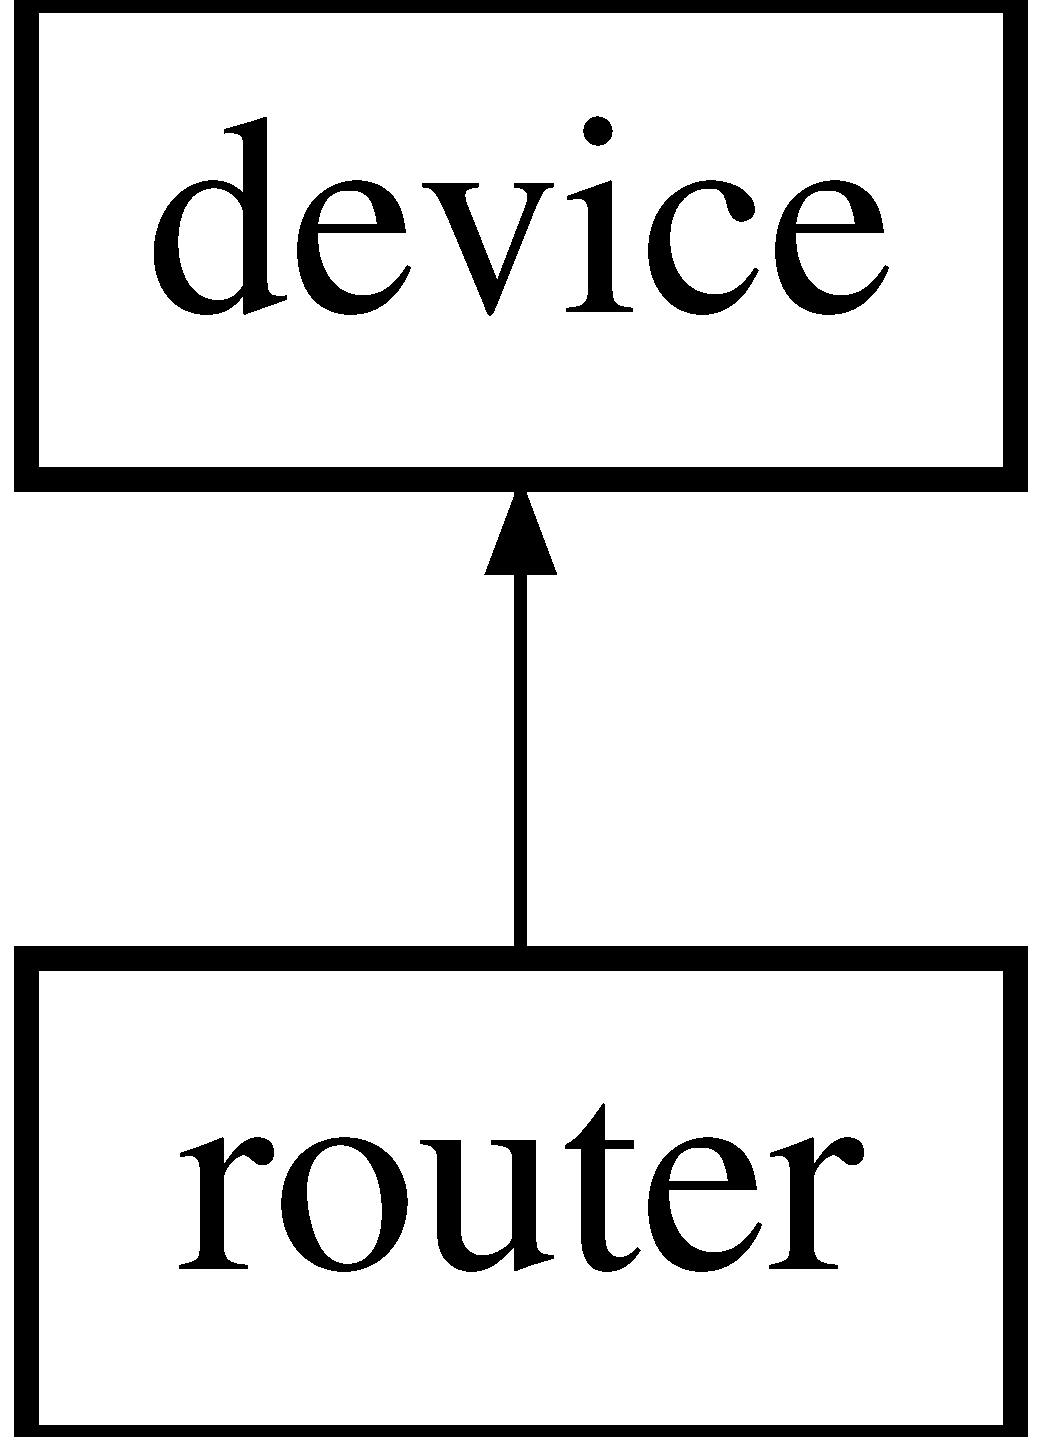
\includegraphics[height=2.000000cm]{classrouter}
\end{center}
\end{figure}
\subsection*{\-Public \-Member \-Functions}
\begin{DoxyCompactItemize}
\item 
\hyperlink{classrouter_af5559739f6e4f9b1c7f7bf80e32f6cd9}{router} ()
\begin{DoxyCompactList}\small\item\em \-Construct empty router. \end{DoxyCompactList}\item 
\hyperlink{classrouter_a43d7888550284a3bffff71abf6c087eb}{router} (int, string, double, double, int, int)
\begin{DoxyCompactList}\small\item\em \-Construct a router. \end{DoxyCompactList}\item 
\hyperlink{classrouter_a64870f29b48d6ee6276ec27b1b18e189}{$\sim$router} ()
\begin{DoxyCompactList}\small\item\em \-Destructor. \end{DoxyCompactList}\item 
list$<$ \hyperlink{classrLink}{r\-Link} $>$ \hyperlink{classrouter_a36115bd5923217c64922b2231f05c304}{get\-R\-List\-Link} ()
\begin{DoxyCompactList}\small\item\em \-Gets a router's link list. \end{DoxyCompactList}\item 
double \hyperlink{classrouter_a0c1d4a7689e992d90b0fcbf4a958c8b4}{get\-Actual\-Capacity} ()
\begin{DoxyCompactList}\small\item\em \-Gets actual capacity of a router. \end{DoxyCompactList}\item 
double \hyperlink{classrouter_a7d5187977fd2dbf2fa562d3953647699}{get\-Residual} ()
\begin{DoxyCompactList}\small\item\em \-Gets residual capacity of a router. \end{DoxyCompactList}\item 
double \hyperlink{classrouter_a425b6d8372b0951a77097d0e6b49914a}{get\-Total\-Power} ()
\begin{DoxyCompactList}\small\item\em \-Get total power of a router = router power + sum of power of the links there of. \end{DoxyCompactList}\item 
bool \hyperlink{classrouter_aaa3d78b2556a095f725d5a2202265d55}{get\-Flag} ()
\begin{DoxyCompactList}\small\item\em \-Gets if a flag is set or not. \end{DoxyCompactList}\item 
void \hyperlink{classrouter_a20f58c16edd3ca8d8afb73cf9f27f549}{set\-L\-List} (\hyperlink{classrLink}{r\-Link})
\begin{DoxyCompactList}\small\item\em \-Sets a router's link list. \end{DoxyCompactList}\item 
void \hyperlink{classrouter_a28908a05b7e50a0ab45481c94c8042a8}{set\-R\-Link\-List} (list$<$ \hyperlink{classrLink}{r\-Link} $>$)
\begin{DoxyCompactList}\small\item\em \-Overwrite a router's link list if required after some modification. \end{DoxyCompactList}\item 
void \hyperlink{classrouter_a90c5339e7bed5597f06be903305ef588}{set\-Actual\-Capacity} (double)
\begin{DoxyCompactList}\small\item\em \-Sets a router's capacity. \end{DoxyCompactList}\item 
void \hyperlink{classrouter_a9b06f4e341fea7bf5a853b0a2caf1d2a}{set\-Total\-Power} (double)
\begin{DoxyCompactList}\small\item\em \-Sets a router's total power consumption = router power + sum of power consumption of links thereof. \end{DoxyCompactList}\item 
void \hyperlink{classrouter_ac839466bae2c42cee73a33b4d185f48a}{set\-Residual} (double)
\begin{DoxyCompactList}\small\item\em \-Sets residual capacity. \end{DoxyCompactList}\item 
void \hyperlink{classrouter_ab4e2af9a6d0412fa8d3e6cea8b411f7c}{set\-Flag} (bool)
\begin{DoxyCompactList}\small\item\em \-Sets/\-Resets router flag. \end{DoxyCompactList}\end{DoxyCompactItemize}


\subsection{\-Detailed \-Description}
\-Multistage architecture router class reference. 

\-It inherits device class and creates a new router with list of links in the same router.

{\bfseries \-Usage \-Example\-:} 
\begin{DoxyCode}
 router *r = new router(1, "router_1", 0, 0, 0, 0)
\end{DoxyCode}
 \begin{DoxySeeAlso}{\-See also}
\hyperlink{classdevice_a57b9c4ac7a8bd970b81b1154ae79a5de}{device(int ,string ,double ,double ,int ,int )} 
\end{DoxySeeAlso}


\subsection{\-Constructor \& \-Destructor \-Documentation}
\hypertarget{classrouter_af5559739f6e4f9b1c7f7bf80e32f6cd9}{\index{router@{router}!router@{router}}
\index{router@{router}!router@{router}}
\subsubsection[{router}]{\setlength{\rightskip}{0pt plus 5cm}{\bf router\-::router} (
\begin{DoxyParamCaption}
{}
\end{DoxyParamCaption}
)\hspace{0.3cm}{\ttfamily  \mbox{[}inline\mbox{]}}}}\label{classrouter_af5559739f6e4f9b1c7f7bf80e32f6cd9}


\-Construct empty router. 

\hypertarget{classrouter_a43d7888550284a3bffff71abf6c087eb}{\index{router@{router}!router@{router}}
\index{router@{router}!router@{router}}
\subsubsection[{router}]{\setlength{\rightskip}{0pt plus 5cm}{\bf router\-::router} (
\begin{DoxyParamCaption}
\item[{int}]{\-I\-D, }
\item[{string}]{name, }
\item[{double}]{capacity, }
\item[{double}]{power, }
\item[{int}]{state, }
\item[{int}]{nr\-\_\-links}
\end{DoxyParamCaption}
)}}\label{classrouter_a43d7888550284a3bffff71abf6c087eb}


\-Construct a router. 


\begin{DoxyParams}{\-Parameters}
{\em \-I\-D} & router identification number \\
\hline
{\em name} & router name \\
\hline
{\em capacity} & router capacity \\
\hline
{\em power} & router power consumption \\
\hline
{\em nr\-\_\-links} & number of links contained inside a router \\
\hline
{\em state} & router state\-: \-O\-N/\-O\-F\-F \\
\hline
\end{DoxyParams}
\begin{DoxySeeAlso}{\-See also}
\hyperlink{classdevice_a57b9c4ac7a8bd970b81b1154ae79a5de}{device(int ,string ,double ,double ,int ,int )} 
\end{DoxySeeAlso}
\hypertarget{classrouter_a64870f29b48d6ee6276ec27b1b18e189}{\index{router@{router}!$\sim$router@{$\sim$router}}
\index{$\sim$router@{$\sim$router}!router@{router}}
\subsubsection[{$\sim$router}]{\setlength{\rightskip}{0pt plus 5cm}{\bf router\-::$\sim$router} (
\begin{DoxyParamCaption}
{}
\end{DoxyParamCaption}
)\hspace{0.3cm}{\ttfamily  \mbox{[}inline\mbox{]}}}}\label{classrouter_a64870f29b48d6ee6276ec27b1b18e189}


\-Destructor. 



\subsection{\-Member \-Function \-Documentation}
\hypertarget{classrouter_a0c1d4a7689e992d90b0fcbf4a958c8b4}{\index{router@{router}!get\-Actual\-Capacity@{get\-Actual\-Capacity}}
\index{get\-Actual\-Capacity@{get\-Actual\-Capacity}!router@{router}}
\subsubsection[{get\-Actual\-Capacity}]{\setlength{\rightskip}{0pt plus 5cm}double {\bf router\-::get\-Actual\-Capacity} (
\begin{DoxyParamCaption}
{}
\end{DoxyParamCaption}
)}}\label{classrouter_a0c1d4a7689e992d90b0fcbf4a958c8b4}


\-Gets actual capacity of a router. 

\begin{DoxyReturn}{\-Returns}
actual capacity of a router 
\end{DoxyReturn}
\hypertarget{classrouter_aaa3d78b2556a095f725d5a2202265d55}{\index{router@{router}!get\-Flag@{get\-Flag}}
\index{get\-Flag@{get\-Flag}!router@{router}}
\subsubsection[{get\-Flag}]{\setlength{\rightskip}{0pt plus 5cm}bool {\bf router\-::get\-Flag} (
\begin{DoxyParamCaption}
{}
\end{DoxyParamCaption}
)}}\label{classrouter_aaa3d78b2556a095f725d5a2202265d55}


\-Gets if a flag is set or not. 

\begin{DoxyReturn}{\-Returns}
usage flag indicator 
\end{DoxyReturn}
\hypertarget{classrouter_a7d5187977fd2dbf2fa562d3953647699}{\index{router@{router}!get\-Residual@{get\-Residual}}
\index{get\-Residual@{get\-Residual}!router@{router}}
\subsubsection[{get\-Residual}]{\setlength{\rightskip}{0pt plus 5cm}double {\bf router\-::get\-Residual} (
\begin{DoxyParamCaption}
{}
\end{DoxyParamCaption}
)}}\label{classrouter_a7d5187977fd2dbf2fa562d3953647699}


\-Gets residual capacity of a router. 

\begin{DoxyReturn}{\-Returns}
residual capacity of a router 
\end{DoxyReturn}
\hypertarget{classrouter_a36115bd5923217c64922b2231f05c304}{\index{router@{router}!get\-R\-List\-Link@{get\-R\-List\-Link}}
\index{get\-R\-List\-Link@{get\-R\-List\-Link}!router@{router}}
\subsubsection[{get\-R\-List\-Link}]{\setlength{\rightskip}{0pt plus 5cm}list$<$ {\bf r\-Link} $>$ {\bf router\-::get\-R\-List\-Link} (
\begin{DoxyParamCaption}
{}
\end{DoxyParamCaption}
)}}\label{classrouter_a36115bd5923217c64922b2231f05c304}


\-Gets a router's link list. 

\begin{DoxyReturn}{\-Returns}
list of links on a router 
\end{DoxyReturn}
\hypertarget{classrouter_a425b6d8372b0951a77097d0e6b49914a}{\index{router@{router}!get\-Total\-Power@{get\-Total\-Power}}
\index{get\-Total\-Power@{get\-Total\-Power}!router@{router}}
\subsubsection[{get\-Total\-Power}]{\setlength{\rightskip}{0pt plus 5cm}double {\bf router\-::get\-Total\-Power} (
\begin{DoxyParamCaption}
{}
\end{DoxyParamCaption}
)}}\label{classrouter_a425b6d8372b0951a77097d0e6b49914a}


\-Get total power of a router = router power + sum of power of the links there of. 

\begin{DoxyReturn}{\-Returns}
total power of a router 
\end{DoxyReturn}
\hypertarget{classrouter_a90c5339e7bed5597f06be903305ef588}{\index{router@{router}!set\-Actual\-Capacity@{set\-Actual\-Capacity}}
\index{set\-Actual\-Capacity@{set\-Actual\-Capacity}!router@{router}}
\subsubsection[{set\-Actual\-Capacity}]{\setlength{\rightskip}{0pt plus 5cm}void {\bf router\-::set\-Actual\-Capacity} (
\begin{DoxyParamCaption}
\item[{double}]{actual\-Capacity}
\end{DoxyParamCaption}
)}}\label{classrouter_a90c5339e7bed5597f06be903305ef588}


\-Sets a router's capacity. 


\begin{DoxyParams}{\-Parameters}
{\em actual\-Capacity} & router capacity \\
\hline
\end{DoxyParams}
\hypertarget{classrouter_ab4e2af9a6d0412fa8d3e6cea8b411f7c}{\index{router@{router}!set\-Flag@{set\-Flag}}
\index{set\-Flag@{set\-Flag}!router@{router}}
\subsubsection[{set\-Flag}]{\setlength{\rightskip}{0pt plus 5cm}void {\bf router\-::set\-Flag} (
\begin{DoxyParamCaption}
\item[{bool}]{flag}
\end{DoxyParamCaption}
)}}\label{classrouter_ab4e2af9a6d0412fa8d3e6cea8b411f7c}


\-Sets/\-Resets router flag. 


\begin{DoxyParams}{\-Parameters}
{\em flag} & a boolean value\-: 1 if the router is used in routing operation, 0 otherwise \\
\hline
\end{DoxyParams}
\hypertarget{classrouter_a20f58c16edd3ca8d8afb73cf9f27f549}{\index{router@{router}!set\-L\-List@{set\-L\-List}}
\index{set\-L\-List@{set\-L\-List}!router@{router}}
\subsubsection[{set\-L\-List}]{\setlength{\rightskip}{0pt plus 5cm}void {\bf router\-::set\-L\-List} (
\begin{DoxyParamCaption}
\item[{{\bf r\-Link}}]{l}
\end{DoxyParamCaption}
)}}\label{classrouter_a20f58c16edd3ca8d8afb73cf9f27f549}


\-Sets a router's link list. 


\begin{DoxyParams}{\-Parameters}
{\em l} & link with all its attributes \\
\hline
\end{DoxyParams}
\hypertarget{classrouter_ac839466bae2c42cee73a33b4d185f48a}{\index{router@{router}!set\-Residual@{set\-Residual}}
\index{set\-Residual@{set\-Residual}!router@{router}}
\subsubsection[{set\-Residual}]{\setlength{\rightskip}{0pt plus 5cm}void {\bf router\-::set\-Residual} (
\begin{DoxyParamCaption}
\item[{double}]{residual}
\end{DoxyParamCaption}
)}}\label{classrouter_ac839466bae2c42cee73a33b4d185f48a}


\-Sets residual capacity. 


\begin{DoxyParams}{\-Parameters}
{\em residual} & \\
\hline
\end{DoxyParams}
\hypertarget{classrouter_a28908a05b7e50a0ab45481c94c8042a8}{\index{router@{router}!set\-R\-Link\-List@{set\-R\-Link\-List}}
\index{set\-R\-Link\-List@{set\-R\-Link\-List}!router@{router}}
\subsubsection[{set\-R\-Link\-List}]{\setlength{\rightskip}{0pt plus 5cm}void {\bf router\-::set\-R\-Link\-List} (
\begin{DoxyParamCaption}
\item[{list$<$ {\bf r\-Link} $>$}]{l\-List}
\end{DoxyParamCaption}
)}}\label{classrouter_a28908a05b7e50a0ab45481c94c8042a8}


\-Overwrite a router's link list if required after some modification. 


\begin{DoxyParams}{\-Parameters}
{\em l\-List} & link list \\
\hline
\end{DoxyParams}
\hypertarget{classrouter_a9b06f4e341fea7bf5a853b0a2caf1d2a}{\index{router@{router}!set\-Total\-Power@{set\-Total\-Power}}
\index{set\-Total\-Power@{set\-Total\-Power}!router@{router}}
\subsubsection[{set\-Total\-Power}]{\setlength{\rightskip}{0pt plus 5cm}void {\bf router\-::set\-Total\-Power} (
\begin{DoxyParamCaption}
\item[{double}]{total\-P}
\end{DoxyParamCaption}
)}}\label{classrouter_a9b06f4e341fea7bf5a853b0a2caf1d2a}


\-Sets a router's total power consumption = router power + sum of power consumption of links thereof. 


\begin{DoxyParams}{\-Parameters}
{\em total\-P} & total power consumption of a router \\
\hline
\end{DoxyParams}


\-The documentation for this class was generated from the following files\-:\begin{DoxyCompactItemize}
\item 
/media/\-Data/research/code/online\-\_\-unsplittable\-\_\-heuristic/include/\hyperlink{router_8h}{router.\-h}\item 
/media/\-Data/research/code/online\-\_\-unsplittable\-\_\-heuristic/\hyperlink{router_8cpp}{router.\-cpp}\end{DoxyCompactItemize}

\hypertarget{classsorter}{
\section{sorter Class Reference}
\label{classsorter}\index{sorter@{sorter}}
}


sort routers and links according to their efficiency; also used to sort the input traffic  




{\ttfamily \#include $<$sorter.h$>$}

\subsection*{Public Member Functions}
\begin{DoxyCompactItemize}
\item 
\hyperlink{classsorter_a0ff82eecc48ab163c3286cee244b7d92}{sorter} ()
\begin{DoxyCompactList}\small\item\em constructor \item\end{DoxyCompactList}\item 
\hyperlink{classsorter_a27f9666807092c172a5ad6f0048d2b57}{$\sim$sorter} ()
\begin{DoxyCompactList}\small\item\em destructor \item\end{DoxyCompactList}\item 
void \hyperlink{classsorter_aa5c4e14df085599365f57f144ffb25be}{rsort} (list$<$ \hyperlink{classrouter}{router} $>$ \&)
\begin{DoxyCompactList}\small\item\em compare each routers with the others First -\/ sort the routers according to: actualCapacity/router power Second -\/ sort the links on each router \item\end{DoxyCompactList}\item 
list$<$ \hyperlink{classrLink}{rLink} $>$ \hyperlink{classsorter_a8c6f644537f597bc5ab57e2012655754}{lsort} (list$<$ \hyperlink{classrLink}{rLink} $>$)
\begin{DoxyCompactList}\small\item\em sorts the links on a router \item\end{DoxyCompactList}\item 
void \hyperlink{classsorter_a4b7e91f19fb0bcb73c1e32d168353b40}{shuffle} (list$<$ \hyperlink{classrouter}{router} $>$ \&)
\begin{DoxyCompactList}\small\item\em shuffle the list of routers and the links thereof \item\end{DoxyCompactList}\item 
void \hyperlink{classsorter_ae5717a09e1732631a6edcf122f2498c5}{tsort} (vector$<$ double $>$ \&)
\begin{DoxyCompactList}\small\item\em sorts the incoming traffic flows \item\end{DoxyCompactList}\end{DoxyCompactItemize}


\subsection{Detailed Description}
sort routers and links according to their efficiency; also used to sort the input traffic After reading the list of routers from a text configuration file, the algorithm sorts the routers according to their efficiency if \_\-ROUTER\_\-POWER\_\-SORT is defined.

Procedure: \begin{DoxyItemize}
\item sort the routers according to (only router power considered for sorting the routers): \begin{eqnarray} \eta_{_{NIC-}} = \frac{C_{r}}{P_{r}} \end{eqnarray} OR (both link and router power considered for sorting the routers) \begin{eqnarray} \eta_{_{NIC+}} = \frac{C_{r}}{P_{r} + \sum_{i=1}^N{P_{rl}}} \end{eqnarray} \item sort the links on each router according to: \begin{eqnarray} \eta_{_l} = \frac{C_{rl}}{P_{rl}} \end{eqnarray} 
\begin{DoxyParams}{Parameters}
\item[{\em rList}]list of routers \end{DoxyParams}
\begin{DoxyReturn}{Returns}
rList ordered list of routers 
\end{DoxyReturn}
\end{DoxyItemize}


\subsection{Constructor \& Destructor Documentation}
\hypertarget{classsorter_a0ff82eecc48ab163c3286cee244b7d92}{
\index{sorter@{sorter}!sorter@{sorter}}
\index{sorter@{sorter}!sorter@{sorter}}
\subsubsection[{sorter}]{\setlength{\rightskip}{0pt plus 5cm}sorter::sorter ()}}
\label{classsorter_a0ff82eecc48ab163c3286cee244b7d92}


constructor 

\hypertarget{classsorter_a27f9666807092c172a5ad6f0048d2b57}{
\index{sorter@{sorter}!$\sim$sorter@{$\sim$sorter}}
\index{$\sim$sorter@{$\sim$sorter}!sorter@{sorter}}
\subsubsection[{$\sim$sorter}]{\setlength{\rightskip}{0pt plus 5cm}sorter::$\sim$sorter ()}}
\label{classsorter_a27f9666807092c172a5ad6f0048d2b57}


destructor 



\subsection{Member Function Documentation}
\hypertarget{classsorter_a8c6f644537f597bc5ab57e2012655754}{
\index{sorter@{sorter}!lsort@{lsort}}
\index{lsort@{lsort}!sorter@{sorter}}
\subsubsection[{lsort}]{\setlength{\rightskip}{0pt plus 5cm}list$<$ {\bf rLink} $>$ sorter::lsort (list$<$ {\bf rLink} $>$ {\em lList})}}
\label{classsorter_a8c6f644537f597bc5ab57e2012655754}


sorts the links on a router 


\begin{DoxyParams}{Parameters}
\item[{\em lList}]list of links to be sorted \end{DoxyParams}
\begin{DoxyReturn}{Returns}
sorted lList 
\end{DoxyReturn}
\hypertarget{classsorter_aa5c4e14df085599365f57f144ffb25be}{
\index{sorter@{sorter}!rsort@{rsort}}
\index{rsort@{rsort}!sorter@{sorter}}
\subsubsection[{rsort}]{\setlength{\rightskip}{0pt plus 5cm}void sorter::rsort (list$<$ {\bf router} $>$ \& {\em rList})}}
\label{classsorter_aa5c4e14df085599365f57f144ffb25be}


compare each routers with the others First -\/ sort the routers according to: actualCapacity/router power Second -\/ sort the links on each router 

\hypertarget{classsorter_a4b7e91f19fb0bcb73c1e32d168353b40}{
\index{sorter@{sorter}!shuffle@{shuffle}}
\index{shuffle@{shuffle}!sorter@{sorter}}
\subsubsection[{shuffle}]{\setlength{\rightskip}{0pt plus 5cm}void sorter::shuffle (list$<$ {\bf router} $>$ \& {\em rList})}}
\label{classsorter_a4b7e91f19fb0bcb73c1e32d168353b40}


shuffle the list of routers and the links thereof 


\begin{DoxyParams}{Parameters}
\item[{\em rList}]list of routers \end{DoxyParams}
\hypertarget{classsorter_ae5717a09e1732631a6edcf122f2498c5}{
\index{sorter@{sorter}!tsort@{tsort}}
\index{tsort@{tsort}!sorter@{sorter}}
\subsubsection[{tsort}]{\setlength{\rightskip}{0pt plus 5cm}void sorter::tsort (vector$<$ double $>$ \& {\em traffic})}}
\label{classsorter_ae5717a09e1732631a6edcf122f2498c5}


sorts the incoming traffic flows 


\begin{DoxyParams}{Parameters}
\item[{\em traffic}]list of traffic flows \end{DoxyParams}
\begin{DoxyReturn}{Returns}
sorted traffic 
\end{DoxyReturn}


The documentation for this class was generated from the following files:\begin{DoxyCompactItemize}
\item 
/media/Data/research/code/online\_\-unsplittable\_\-heuristic/include/\hyperlink{sorter_8h}{sorter.h}\item 
/media/Data/research/code/online\_\-unsplittable\_\-heuristic/\hyperlink{sorter_8cpp}{sorter.cpp}\end{DoxyCompactItemize}

\hypertarget{classstatistics}{
\section{statistics Class Reference}
\label{classstatistics}\index{statistics@{statistics}}
}


Statistics class to collect device states.  




{\ttfamily \#include $<$statistics.h$>$}

\subsection*{Public Member Functions}
\begin{DoxyCompactItemize}
\item 
\hyperlink{classstatistics_a31d6750c3251c979f5c2d013984e1162}{statistics} ()
\begin{DoxyCompactList}\small\item\em constructor \item\end{DoxyCompactList}\item 
\hyperlink{classstatistics_a8cf720227802726be118712dc6616f94}{$\sim$statistics} ()
\begin{DoxyCompactList}\small\item\em destructor \item\end{DoxyCompactList}\item 
std::vector$<$ double $>$ \hyperlink{classstatistics_ab2c51b1a4cc826a09473860faf565360}{getForwardedList} ()
\begin{DoxyCompactList}\small\item\em get forwarded traffic list \item\end{DoxyCompactList}\item 
std::vector$<$ double $>$ \hyperlink{classstatistics_a99795974e97556668c02c5005b2df895}{getLostList} ()
\begin{DoxyCompactList}\small\item\em get lost traffic list \item\end{DoxyCompactList}\item 
std::vector$<$ long $>$ \hyperlink{classstatistics_a857adb219cf897c105a9e0aceca4188a}{getTimeAdvList} ()
\begin{DoxyCompactList}\small\item\em get advanced time \item\end{DoxyCompactList}\item 
std::vector$<$ double $>$ \hyperlink{classstatistics_a47b6c911143330c41faa573bc534aee1}{getObjectiveList} ()
\begin{DoxyCompactList}\small\item\em get objective \item\end{DoxyCompactList}\item 
std::vector$<$ double $>$ \hyperlink{classstatistics_a170d529ea5d3c459755309e2de1d166e}{getLoadList} ()
\begin{DoxyCompactList}\small\item\em get load \item\end{DoxyCompactList}\item 
double \hyperlink{classstatistics_a8a09566df54f2ac183e0a40f452546a6}{getObjective} ()
\begin{DoxyCompactList}\small\item\em get objective previous \item\end{DoxyCompactList}\item 
std::vector$<$ double $>$ \hyperlink{classstatistics_af512ba48d195d791b927bc49e2c40188}{getTraffic} ()
\begin{DoxyCompactList}\small\item\em get traffic statistics \item\end{DoxyCompactList}\item 
std::vector$<$ double $>$ \hyperlink{classstatistics_a7aa58e77f08e583a87f9050a5b1cf4f9}{getTrafficDiff} ()
\begin{DoxyCompactList}\small\item\em get traffic difference between current and previous traffic \item\end{DoxyCompactList}\item 
void \hyperlink{classstatistics_a94f979fcc6d511583638d6fc12116992}{setForwardedList} (double)
\begin{DoxyCompactList}\small\item\em set forwarded traffic list \item\end{DoxyCompactList}\item 
void \hyperlink{classstatistics_a84bead3d62e23af1777b5e54c6de48de}{setLostList} (double)
\begin{DoxyCompactList}\small\item\em set lost traffic list \item\end{DoxyCompactList}\item 
void \hyperlink{classstatistics_ab2fd434123379e7814c21bc38ff2bb20}{setObjective} (double)
\begin{DoxyCompactList}\small\item\em set current objective \item\end{DoxyCompactList}\item 
void \hyperlink{classstatistics_a625258dee0b4eaf0fa5ade3643a4535e}{setObjectiveList} (double)
\begin{DoxyCompactList}\small\item\em put objective in the list \item\end{DoxyCompactList}\item 
void \hyperlink{classstatistics_af1594f7585e2c0776ef2f8fb7ddd3fca}{setLoadList} (double)
\begin{DoxyCompactList}\small\item\em set load \item\end{DoxyCompactList}\item 
void \hyperlink{classstatistics_aa371004886cf08d7632027c575d983fc}{clearForwardList} ()
\begin{DoxyCompactList}\small\item\em clear the forwarded traffic list \item\end{DoxyCompactList}\item 
void \hyperlink{classstatistics_a897546605e8b6c2b2ec411092e89dab8}{clearLostList} ()
\begin{DoxyCompactList}\small\item\em clear the lost traffic list \item\end{DoxyCompactList}\item 
void \hyperlink{classstatistics_a3eca72da112aae2a944b7dc40a59b787}{setTraffic} (std::vector$<$ double $>$ newTraffic)
\begin{DoxyCompactList}\small\item\em set current traffic \item\end{DoxyCompactList}\item 
void \hyperlink{classstatistics_ae5d56a6dc6878004b42d10369de284de}{setTrafficPrev} (std::vector$<$ double $>$ prevTraffic)
\begin{DoxyCompactList}\small\item\em set previous traffic \item\end{DoxyCompactList}\end{DoxyCompactItemize}


\subsection{Detailed Description}
Statistics class to collect device states. General traffic statistics -\/ such as lost traffic, total forwarded traffic, total power consumption (objective) 

\subsection{Constructor \& Destructor Documentation}
\hypertarget{classstatistics_a31d6750c3251c979f5c2d013984e1162}{
\index{statistics@{statistics}!statistics@{statistics}}
\index{statistics@{statistics}!statistics@{statistics}}
\subsubsection[{statistics}]{\setlength{\rightskip}{0pt plus 5cm}statistics::statistics ()}}
\label{classstatistics_a31d6750c3251c979f5c2d013984e1162}


constructor 

\hypertarget{classstatistics_a8cf720227802726be118712dc6616f94}{
\index{statistics@{statistics}!$\sim$statistics@{$\sim$statistics}}
\index{$\sim$statistics@{$\sim$statistics}!statistics@{statistics}}
\subsubsection[{$\sim$statistics}]{\setlength{\rightskip}{0pt plus 5cm}statistics::$\sim$statistics ()\hspace{0.3cm}{\ttfamily  \mbox{[}inline\mbox{]}}}}
\label{classstatistics_a8cf720227802726be118712dc6616f94}


destructor 



\subsection{Member Function Documentation}
\hypertarget{classstatistics_aa371004886cf08d7632027c575d983fc}{
\index{statistics@{statistics}!clearForwardList@{clearForwardList}}
\index{clearForwardList@{clearForwardList}!statistics@{statistics}}
\subsubsection[{clearForwardList}]{\setlength{\rightskip}{0pt plus 5cm}void statistics::clearForwardList ()}}
\label{classstatistics_aa371004886cf08d7632027c575d983fc}


clear the forwarded traffic list 

\hypertarget{classstatistics_a897546605e8b6c2b2ec411092e89dab8}{
\index{statistics@{statistics}!clearLostList@{clearLostList}}
\index{clearLostList@{clearLostList}!statistics@{statistics}}
\subsubsection[{clearLostList}]{\setlength{\rightskip}{0pt plus 5cm}void statistics::clearLostList ()}}
\label{classstatistics_a897546605e8b6c2b2ec411092e89dab8}


clear the lost traffic list 

\hypertarget{classstatistics_ab2c51b1a4cc826a09473860faf565360}{
\index{statistics@{statistics}!getForwardedList@{getForwardedList}}
\index{getForwardedList@{getForwardedList}!statistics@{statistics}}
\subsubsection[{getForwardedList}]{\setlength{\rightskip}{0pt plus 5cm}std::vector$<$ double $>$ statistics::getForwardedList ()}}
\label{classstatistics_ab2c51b1a4cc826a09473860faf565360}


get forwarded traffic list 

\begin{DoxyReturn}{Returns}
forwarded traffic list 
\end{DoxyReturn}
\hypertarget{classstatistics_a170d529ea5d3c459755309e2de1d166e}{
\index{statistics@{statistics}!getLoadList@{getLoadList}}
\index{getLoadList@{getLoadList}!statistics@{statistics}}
\subsubsection[{getLoadList}]{\setlength{\rightskip}{0pt plus 5cm}std::vector$<$ double $>$ statistics::getLoadList ()}}
\label{classstatistics_a170d529ea5d3c459755309e2de1d166e}


get load 

\begin{DoxyReturn}{Returns}
list of loads 
\end{DoxyReturn}
\hypertarget{classstatistics_a99795974e97556668c02c5005b2df895}{
\index{statistics@{statistics}!getLostList@{getLostList}}
\index{getLostList@{getLostList}!statistics@{statistics}}
\subsubsection[{getLostList}]{\setlength{\rightskip}{0pt plus 5cm}std::vector$<$ double $>$ statistics::getLostList ()}}
\label{classstatistics_a99795974e97556668c02c5005b2df895}


get lost traffic list 

\begin{DoxyReturn}{Returns}
lost traffic list 
\end{DoxyReturn}
\hypertarget{classstatistics_a8a09566df54f2ac183e0a40f452546a6}{
\index{statistics@{statistics}!getObjective@{getObjective}}
\index{getObjective@{getObjective}!statistics@{statistics}}
\subsubsection[{getObjective}]{\setlength{\rightskip}{0pt plus 5cm}double statistics::getObjective ()}}
\label{classstatistics_a8a09566df54f2ac183e0a40f452546a6}


get objective previous 

\begin{DoxyReturn}{Returns}
total power consumption of the previous configuration of the architecture 
\end{DoxyReturn}
\hypertarget{classstatistics_a47b6c911143330c41faa573bc534aee1}{
\index{statistics@{statistics}!getObjectiveList@{getObjectiveList}}
\index{getObjectiveList@{getObjectiveList}!statistics@{statistics}}
\subsubsection[{getObjectiveList}]{\setlength{\rightskip}{0pt plus 5cm}std::vector$<$ double $>$ statistics::getObjectiveList ()}}
\label{classstatistics_a47b6c911143330c41faa573bc534aee1}


get objective 

\begin{DoxyReturn}{Returns}
list of total power consumption of the architecture 
\end{DoxyReturn}
\hypertarget{classstatistics_a857adb219cf897c105a9e0aceca4188a}{
\index{statistics@{statistics}!getTimeAdvList@{getTimeAdvList}}
\index{getTimeAdvList@{getTimeAdvList}!statistics@{statistics}}
\subsubsection[{getTimeAdvList}]{\setlength{\rightskip}{0pt plus 5cm}std::vector$<$long$>$ statistics::getTimeAdvList ()}}
\label{classstatistics_a857adb219cf897c105a9e0aceca4188a}


get advanced time 

\begin{DoxyReturn}{Returns}
time required for packing 
\end{DoxyReturn}
\hypertarget{classstatistics_af512ba48d195d791b927bc49e2c40188}{
\index{statistics@{statistics}!getTraffic@{getTraffic}}
\index{getTraffic@{getTraffic}!statistics@{statistics}}
\subsubsection[{getTraffic}]{\setlength{\rightskip}{0pt plus 5cm}std::vector$<$ double $>$ statistics::getTraffic ()}}
\label{classstatistics_af512ba48d195d791b927bc49e2c40188}


get traffic statistics 

\hypertarget{classstatistics_a7aa58e77f08e583a87f9050a5b1cf4f9}{
\index{statistics@{statistics}!getTrafficDiff@{getTrafficDiff}}
\index{getTrafficDiff@{getTrafficDiff}!statistics@{statistics}}
\subsubsection[{getTrafficDiff}]{\setlength{\rightskip}{0pt plus 5cm}vector$<$ double $>$ statistics::getTrafficDiff ()}}
\label{classstatistics_a7aa58e77f08e583a87f9050a5b1cf4f9}


get traffic difference between current and previous traffic 

\hypertarget{classstatistics_a94f979fcc6d511583638d6fc12116992}{
\index{statistics@{statistics}!setForwardedList@{setForwardedList}}
\index{setForwardedList@{setForwardedList}!statistics@{statistics}}
\subsubsection[{setForwardedList}]{\setlength{\rightskip}{0pt plus 5cm}void statistics::setForwardedList (double {\em forwarded})}}
\label{classstatistics_a94f979fcc6d511583638d6fc12116992}


set forwarded traffic list 


\begin{DoxyParams}{Parameters}
\item[{\em forwarded}]routed traffic \end{DoxyParams}
\hypertarget{classstatistics_af1594f7585e2c0776ef2f8fb7ddd3fca}{
\index{statistics@{statistics}!setLoadList@{setLoadList}}
\index{setLoadList@{setLoadList}!statistics@{statistics}}
\subsubsection[{setLoadList}]{\setlength{\rightskip}{0pt plus 5cm}void statistics::setLoadList (double {\em load})}}
\label{classstatistics_af1594f7585e2c0776ef2f8fb7ddd3fca}


set load 


\begin{DoxyParams}{Parameters}
\item[{\em load}]current traffic amount to be forwarded \end{DoxyParams}
\hypertarget{classstatistics_a84bead3d62e23af1777b5e54c6de48de}{
\index{statistics@{statistics}!setLostList@{setLostList}}
\index{setLostList@{setLostList}!statistics@{statistics}}
\subsubsection[{setLostList}]{\setlength{\rightskip}{0pt plus 5cm}void statistics::setLostList (double {\em lost})}}
\label{classstatistics_a84bead3d62e23af1777b5e54c6de48de}


set lost traffic list 


\begin{DoxyParams}{Parameters}
\item[{\em lost}]traffic that is not routed because of lack of capacity \end{DoxyParams}
\hypertarget{classstatistics_ab2fd434123379e7814c21bc38ff2bb20}{
\index{statistics@{statistics}!setObjective@{setObjective}}
\index{setObjective@{setObjective}!statistics@{statistics}}
\subsubsection[{setObjective}]{\setlength{\rightskip}{0pt plus 5cm}void statistics::setObjective (double {\em objective})}}
\label{classstatistics_ab2fd434123379e7814c21bc38ff2bb20}


set current objective 


\begin{DoxyParams}{Parameters}
\item[{\em objective}]power consumption of current configuration \end{DoxyParams}
\hypertarget{classstatistics_a625258dee0b4eaf0fa5ade3643a4535e}{
\index{statistics@{statistics}!setObjectiveList@{setObjectiveList}}
\index{setObjectiveList@{setObjectiveList}!statistics@{statistics}}
\subsubsection[{setObjectiveList}]{\setlength{\rightskip}{0pt plus 5cm}void statistics::setObjectiveList (double {\em objective})}}
\label{classstatistics_a625258dee0b4eaf0fa5ade3643a4535e}


put objective in the list 


\begin{DoxyParams}{Parameters}
\item[{\em objective}]power consumption of current configuration \end{DoxyParams}
\hypertarget{classstatistics_a3eca72da112aae2a944b7dc40a59b787}{
\index{statistics@{statistics}!setTraffic@{setTraffic}}
\index{setTraffic@{setTraffic}!statistics@{statistics}}
\subsubsection[{setTraffic}]{\setlength{\rightskip}{0pt plus 5cm}void statistics::setTraffic (std::vector$<$ double $>$ {\em newTraffic})}}
\label{classstatistics_a3eca72da112aae2a944b7dc40a59b787}


set current traffic 


\begin{DoxyParams}{Parameters}
\item[{\em newTraffic}]input traffic \end{DoxyParams}
\hypertarget{classstatistics_ae5d56a6dc6878004b42d10369de284de}{
\index{statistics@{statistics}!setTrafficPrev@{setTrafficPrev}}
\index{setTrafficPrev@{setTrafficPrev}!statistics@{statistics}}
\subsubsection[{setTrafficPrev}]{\setlength{\rightskip}{0pt plus 5cm}void statistics::setTrafficPrev (std::vector$<$ double $>$ {\em prevTraffic})}}
\label{classstatistics_ae5d56a6dc6878004b42d10369de284de}


set previous traffic 


\begin{DoxyParams}{Parameters}
\item[{\em prevTraffic}]input traffic \end{DoxyParams}


The documentation for this class was generated from the following files:\begin{DoxyCompactItemize}
\item 
/media/Data/research/code/online\_\-unsplittable\_\-heuristic/include/\hyperlink{statistics_8h}{statistics.h}\item 
/media/Data/research/code/online\_\-unsplittable\_\-heuristic/\hyperlink{statistics_8cpp}{statistics.cpp}\end{DoxyCompactItemize}

\chapter{File Documentation}
\hypertarget{device_8cpp}{\section{/media/\-Data/research/code/online\-\_\-unsplittable\-\_\-heuristic/device.cpp \-File \-Reference}
\label{device_8cpp}\index{/media/\-Data/research/code/online\-\_\-unsplittable\-\_\-heuristic/device.\-cpp@{/media/\-Data/research/code/online\-\_\-unsplittable\-\_\-heuristic/device.\-cpp}}
}
{\ttfamily \#include \char`\"{}device.\-h\char`\"{}}\*
{\ttfamily \#include \char`\"{}global.\-h\char`\"{}}\*
{\ttfamily \#include $<$string$>$}\*
{\ttfamily \#include $<$iostream$>$}\*
{\ttfamily \#include $<$vector$>$}\*

\hypertarget{deviceSetup_8cpp}{
\section{/media/Data/research/code/online\_\-unsplittable\_\-heuristic/deviceSetup.cpp File Reference}
\label{deviceSetup_8cpp}\index{/media/Data/research/code/online\_\-unsplittable\_\-heuristic/deviceSetup.cpp@{/media/Data/research/code/online\_\-unsplittable\_\-heuristic/deviceSetup.cpp}}
}
{\ttfamily \#include \char`\"{}deviceSetup.h\char`\"{}}\par
{\ttfamily \#include \char`\"{}global.h\char`\"{}}\par
\subsection*{Variables}
\begin{DoxyCompactItemize}
\item 
list$<$ \hyperlink{classrLink}{rLink} $>$ \hyperlink{deviceSetup_8cpp_af9e84ea24bf6207e0d3ac5eade613e49}{lList}
\end{DoxyCompactItemize}


\subsection{Variable Documentation}
\hypertarget{deviceSetup_8cpp_af9e84ea24bf6207e0d3ac5eade613e49}{
\index{deviceSetup.cpp@{deviceSetup.cpp}!lList@{lList}}
\index{lList@{lList}!deviceSetup.cpp@{deviceSetup.cpp}}
\subsubsection[{lList}]{\setlength{\rightskip}{0pt plus 5cm}list$<${\bf rLink}$>$ {\bf lList}}}
\label{deviceSetup_8cpp_af9e84ea24bf6207e0d3ac5eade613e49}

\hypertarget{device_8h}{\section{/media/\-Data/research/code/online\-\_\-unsplittable\-\_\-heuristic/include/device.h \-File \-Reference}
\label{device_8h}\index{/media/\-Data/research/code/online\-\_\-unsplittable\-\_\-heuristic/include/device.\-h@{/media/\-Data/research/code/online\-\_\-unsplittable\-\_\-heuristic/include/device.\-h}}
}
{\ttfamily \#include $<$string$>$}\*
\subsection*{\-Classes}
\begin{DoxyCompactItemize}
\item 
class \hyperlink{classdevice}{device}
\begin{DoxyCompactList}\small\item\em \-Basic class for devices in the multistage architecture. \end{DoxyCompactList}\end{DoxyCompactItemize}

\hypertarget{deviceSetup_8h}{
\section{/media/Data/research/code/online\_\-unsplittable\_\-heuristic/include/deviceSetup.h File Reference}
\label{deviceSetup_8h}\index{/media/Data/research/code/online\_\-unsplittable\_\-heuristic/include/deviceSetup.h@{/media/Data/research/code/online\_\-unsplittable\_\-heuristic/include/deviceSetup.h}}
}
{\ttfamily \#include \char`\"{}global.h\char`\"{}}\par
{\ttfamily \#include $<$vector$>$}\par
{\ttfamily \#include $<$list$>$}\par
{\ttfamily \#include $<$string$>$}\par
{\ttfamily \#include \char`\"{}device.h\char`\"{}}\par
{\ttfamily \#include \char`\"{}statistics.h\char`\"{}}\par
{\ttfamily \#include \char`\"{}router.h\char`\"{}}\par
{\ttfamily \#include $<$sys/time.h$>$}\par
{\ttfamily \#include $<$iostream$>$}\par
{\ttfamily \#include $<$stdlib.h$>$}\par
{\ttfamily \#include $<$fstream$>$}\par
{\ttfamily \#include \char`\"{}global.h\char`\"{}}\par
\subsection*{Classes}
\begin{DoxyCompactItemize}
\item 
class \hyperlink{classdeviceSetup}{deviceSetup}
\begin{DoxyCompactList}\small\item\em sets up the multistage architecture configuration \item\end{DoxyCompactList}\end{DoxyCompactItemize}

\hypertarget{global_8h}{\section{/media/\-Data/research/code/online\-\_\-unsplittable\-\_\-heuristic/include/global.h \-File \-Reference}
\label{global_8h}\index{/media/\-Data/research/code/online\-\_\-unsplittable\-\_\-heuristic/include/global.\-h@{/media/\-Data/research/code/online\-\_\-unsplittable\-\_\-heuristic/include/global.\-h}}
}
{\ttfamily \#include $<$vector$>$}\*
{\ttfamily \#include $<$list$>$}\*
{\ttfamily \#include \char`\"{}router.\-h\char`\"{}}\*
{\ttfamily \#include \char`\"{}statistics.\-h\char`\"{}}\*
{\ttfamily \#include \char`\"{}multistage.\-h\char`\"{}}\*
{\ttfamily \#include \char`\"{}measurement.\-h\char`\"{}}\*
{\ttfamily \#include \char`\"{}device\-Setup.\-h\char`\"{}}\*
{\ttfamily \#include \char`\"{}parser.\-h\char`\"{}}\*
{\ttfamily \#include \char`\"{}sorter.\-h\char`\"{}}\*
{\ttfamily \#include \char`\"{}packing.\-h\char`\"{}}\*
\subsection*{\-Defines}
\begin{DoxyCompactItemize}
\item 
\#define \hyperlink{global_8h_a4b069399b49024fe80d155d22c2b6c1b}{\-\_\-\-R\-O\-U\-T\-E\-R}
\item 
\#define \hyperlink{global_8h_a0f16e52e3217fbfc0adb34a06cbc3621}{\-\_\-\-R\-E\-S\-U\-L\-T}
\begin{DoxyCompactList}\small\item\em to display some results to see if the algorithm is working properly or not \end{DoxyCompactList}\item 
\#define \hyperlink{global_8h_a36c17f10ff1ad652b64d3fea7d1a01f7}{\-\_\-\-L\-I\-N\-K\-\_\-\-R\-O\-U\-T\-E\-R\-\_\-\-P\-O\-W\-E\-R\-\_\-\-S\-O\-R\-T}
\begin{DoxyCompactList}\small\item\em consider both link and router power consumption in ordering the routers \end{DoxyCompactList}\item 
\#define \hyperlink{global_8h_ad1c3ebe51e1dbc1f2a7d5ea13a12407e}{\-\_\-\-F\-I\-R\-S\-T\-\_\-\-F\-I\-T}
\begin{DoxyCompactList}\small\item\em first fit algorithm \end{DoxyCompactList}\end{DoxyCompactItemize}
\subsection*{\-Functions}
\begin{DoxyCompactItemize}
\item 
void \hyperlink{global_8h_a77899fcfaf7ced1f39a1174db191afd7}{free\-\_\-mem} (\hyperlink{classmultistage}{multistage} $\ast$)
\end{DoxyCompactItemize}
\subsection*{\-Variables}
\begin{DoxyCompactItemize}
\item 
const int \hyperlink{global_8h_a23c002e697540747a04aa4ee0263cbd6}{\-L\-\_\-\-M\-A\-X\-\_\-\-C\-A\-P\-A\-C\-I\-T\-Y} = 800
\begin{DoxyCompactList}\small\item\em possible max link capacity \end{DoxyCompactList}\item 
const int \hyperlink{global_8h_a642f61aabe37e509cb024dda58d48099}{\-L\-\_\-\-M\-I\-N\-\_\-\-C\-A\-P\-A\-C\-I\-T\-Y} = 80
\begin{DoxyCompactList}\small\item\em possible min link capacity \end{DoxyCompactList}\item 
int \hyperlink{global_8h_a14328a11ac1e9bc5a669e2d0341e2f54}{nr\-\_\-flows}
\begin{DoxyCompactList}\small\item\em nr of traffic flows \end{DoxyCompactList}\item 
int \hyperlink{global_8h_ac430c7b9fb12fc01885b9465364e3d97}{nr\-\_\-routers}
\begin{DoxyCompactList}\small\item\em nr of routers in the architecture \end{DoxyCompactList}\item 
int \hyperlink{global_8h_a3288b1e9f09032f99fdd54cfd4a26aa9}{nr\-\_\-links}
\begin{DoxyCompactList}\small\item\em nr of links in a router \end{DoxyCompactList}\item 
vector$<$ double $>$ \hyperlink{global_8h_a49482e053b5a87760f4c3fe1242cd72b}{traffic}
\begin{DoxyCompactList}\small\item\em traffic needed to be routed \end{DoxyCompactList}\item 
vector$<$ double $>$ \hyperlink{global_8h_a1299d2dbbe6f58ee6229ef30aa5f5bde}{r\-\_\-capacity}
\begin{DoxyCompactList}\small\item\em vector of capacity for each router \end{DoxyCompactList}\item 
vector$<$ double $>$ \hyperlink{global_8h_a5b014c61c7abb7b5d95080985d3d2448}{r\-\_\-power}
\begin{DoxyCompactList}\small\item\em vector of power consumption for each router \end{DoxyCompactList}\item 
vector$<$ double $>$ \hyperlink{global_8h_a04f7d3c356c598431b28151df15c7a1e}{l\-\_\-capacity}
\begin{DoxyCompactList}\small\item\em vector of capacity for each link on a router \end{DoxyCompactList}\item 
vector$<$ double $>$ \hyperlink{global_8h_a219826526adf24ccd45b45e6ceab2359}{l\-\_\-power}
\begin{DoxyCompactList}\small\item\em vector of power consumption of each link on a router \end{DoxyCompactList}\item 
vector$<$ vector$<$ double $>$ $>$ \hyperlink{global_8h_a33ae934d11ad20d1de64a6d9aba13623}{all\-\_\-l\-\_\-capacity}
\begin{DoxyCompactList}\small\item\em vector of links on all routers \end{DoxyCompactList}\item 
vector$<$ vector$<$ double $>$ $>$ \hyperlink{global_8h_a62fe6a3c0e8a9ee6c84275f3a2bb0e79}{all\-\_\-l\-\_\-power}
\begin{DoxyCompactList}\small\item\em vector of power consumption of links on all routers \end{DoxyCompactList}\end{DoxyCompactItemize}


\subsection{\-Detailed \-Description}


\subsection{\-Define \-Documentation}
\hypertarget{global_8h_ad1c3ebe51e1dbc1f2a7d5ea13a12407e}{\index{global.\-h@{global.\-h}!\-\_\-\-F\-I\-R\-S\-T\-\_\-\-F\-I\-T@{\-\_\-\-F\-I\-R\-S\-T\-\_\-\-F\-I\-T}}
\index{\-\_\-\-F\-I\-R\-S\-T\-\_\-\-F\-I\-T@{\-\_\-\-F\-I\-R\-S\-T\-\_\-\-F\-I\-T}!global.h@{global.\-h}}
\subsubsection[{\-\_\-\-F\-I\-R\-S\-T\-\_\-\-F\-I\-T}]{\setlength{\rightskip}{0pt plus 5cm}\#define {\bf \-\_\-\-F\-I\-R\-S\-T\-\_\-\-F\-I\-T}}}\label{global_8h_ad1c3ebe51e1dbc1f2a7d5ea13a12407e}


first fit algorithm 

\hypertarget{global_8h_a36c17f10ff1ad652b64d3fea7d1a01f7}{\index{global.\-h@{global.\-h}!\-\_\-\-L\-I\-N\-K\-\_\-\-R\-O\-U\-T\-E\-R\-\_\-\-P\-O\-W\-E\-R\-\_\-\-S\-O\-R\-T@{\-\_\-\-L\-I\-N\-K\-\_\-\-R\-O\-U\-T\-E\-R\-\_\-\-P\-O\-W\-E\-R\-\_\-\-S\-O\-R\-T}}
\index{\-\_\-\-L\-I\-N\-K\-\_\-\-R\-O\-U\-T\-E\-R\-\_\-\-P\-O\-W\-E\-R\-\_\-\-S\-O\-R\-T@{\-\_\-\-L\-I\-N\-K\-\_\-\-R\-O\-U\-T\-E\-R\-\_\-\-P\-O\-W\-E\-R\-\_\-\-S\-O\-R\-T}!global.h@{global.\-h}}
\subsubsection[{\-\_\-\-L\-I\-N\-K\-\_\-\-R\-O\-U\-T\-E\-R\-\_\-\-P\-O\-W\-E\-R\-\_\-\-S\-O\-R\-T}]{\setlength{\rightskip}{0pt plus 5cm}\#define {\bf \-\_\-\-L\-I\-N\-K\-\_\-\-R\-O\-U\-T\-E\-R\-\_\-\-P\-O\-W\-E\-R\-\_\-\-S\-O\-R\-T}}}\label{global_8h_a36c17f10ff1ad652b64d3fea7d1a01f7}


consider both link and router power consumption in ordering the routers 

\hypertarget{global_8h_a0f16e52e3217fbfc0adb34a06cbc3621}{\index{global.\-h@{global.\-h}!\-\_\-\-R\-E\-S\-U\-L\-T@{\-\_\-\-R\-E\-S\-U\-L\-T}}
\index{\-\_\-\-R\-E\-S\-U\-L\-T@{\-\_\-\-R\-E\-S\-U\-L\-T}!global.h@{global.\-h}}
\subsubsection[{\-\_\-\-R\-E\-S\-U\-L\-T}]{\setlength{\rightskip}{0pt plus 5cm}\#define {\bf \-\_\-\-R\-E\-S\-U\-L\-T}}}\label{global_8h_a0f16e52e3217fbfc0adb34a06cbc3621}


to display some results to see if the algorithm is working properly or not 

\hypertarget{global_8h_a4b069399b49024fe80d155d22c2b6c1b}{\index{global.\-h@{global.\-h}!\-\_\-\-R\-O\-U\-T\-E\-R@{\-\_\-\-R\-O\-U\-T\-E\-R}}
\index{\-\_\-\-R\-O\-U\-T\-E\-R@{\-\_\-\-R\-O\-U\-T\-E\-R}!global.h@{global.\-h}}
\subsubsection[{\-\_\-\-R\-O\-U\-T\-E\-R}]{\setlength{\rightskip}{0pt plus 5cm}\#define {\bf \-\_\-\-R\-O\-U\-T\-E\-R}}}\label{global_8h_a4b069399b49024fe80d155d22c2b6c1b}


\subsection{\-Function \-Documentation}
\hypertarget{global_8h_a77899fcfaf7ced1f39a1174db191afd7}{\index{global.\-h@{global.\-h}!free\-\_\-mem@{free\-\_\-mem}}
\index{free\-\_\-mem@{free\-\_\-mem}!global.h@{global.\-h}}
\subsubsection[{free\-\_\-mem}]{\setlength{\rightskip}{0pt plus 5cm}void {\bf free\-\_\-mem} (
\begin{DoxyParamCaption}
\item[{{\bf multistage} $\ast$}]{}
\end{DoxyParamCaption}
)}}\label{global_8h_a77899fcfaf7ced1f39a1174db191afd7}


\subsection{\-Variable \-Documentation}
\hypertarget{global_8h_a33ae934d11ad20d1de64a6d9aba13623}{\index{global.\-h@{global.\-h}!all\-\_\-l\-\_\-capacity@{all\-\_\-l\-\_\-capacity}}
\index{all\-\_\-l\-\_\-capacity@{all\-\_\-l\-\_\-capacity}!global.h@{global.\-h}}
\subsubsection[{all\-\_\-l\-\_\-capacity}]{\setlength{\rightskip}{0pt plus 5cm}vector$<$vector $<$double$>$ $>$ {\bf all\-\_\-l\-\_\-capacity}}}\label{global_8h_a33ae934d11ad20d1de64a6d9aba13623}


vector of links on all routers 

\hypertarget{global_8h_a62fe6a3c0e8a9ee6c84275f3a2bb0e79}{\index{global.\-h@{global.\-h}!all\-\_\-l\-\_\-power@{all\-\_\-l\-\_\-power}}
\index{all\-\_\-l\-\_\-power@{all\-\_\-l\-\_\-power}!global.h@{global.\-h}}
\subsubsection[{all\-\_\-l\-\_\-power}]{\setlength{\rightskip}{0pt plus 5cm}vector$<$vector $<$double$>$ $>$ {\bf all\-\_\-l\-\_\-power}}}\label{global_8h_a62fe6a3c0e8a9ee6c84275f3a2bb0e79}


vector of power consumption of links on all routers 

\hypertarget{global_8h_a04f7d3c356c598431b28151df15c7a1e}{\index{global.\-h@{global.\-h}!l\-\_\-capacity@{l\-\_\-capacity}}
\index{l\-\_\-capacity@{l\-\_\-capacity}!global.h@{global.\-h}}
\subsubsection[{l\-\_\-capacity}]{\setlength{\rightskip}{0pt plus 5cm}vector$<$double$>$ {\bf l\-\_\-capacity}}}\label{global_8h_a04f7d3c356c598431b28151df15c7a1e}


vector of capacity for each link on a router 

\hypertarget{global_8h_a23c002e697540747a04aa4ee0263cbd6}{\index{global.\-h@{global.\-h}!\-L\-\_\-\-M\-A\-X\-\_\-\-C\-A\-P\-A\-C\-I\-T\-Y@{\-L\-\_\-\-M\-A\-X\-\_\-\-C\-A\-P\-A\-C\-I\-T\-Y}}
\index{\-L\-\_\-\-M\-A\-X\-\_\-\-C\-A\-P\-A\-C\-I\-T\-Y@{\-L\-\_\-\-M\-A\-X\-\_\-\-C\-A\-P\-A\-C\-I\-T\-Y}!global.h@{global.\-h}}
\subsubsection[{\-L\-\_\-\-M\-A\-X\-\_\-\-C\-A\-P\-A\-C\-I\-T\-Y}]{\setlength{\rightskip}{0pt plus 5cm}const int {\bf \-L\-\_\-\-M\-A\-X\-\_\-\-C\-A\-P\-A\-C\-I\-T\-Y} = 800}}\label{global_8h_a23c002e697540747a04aa4ee0263cbd6}


possible max link capacity 

\hypertarget{global_8h_a642f61aabe37e509cb024dda58d48099}{\index{global.\-h@{global.\-h}!\-L\-\_\-\-M\-I\-N\-\_\-\-C\-A\-P\-A\-C\-I\-T\-Y@{\-L\-\_\-\-M\-I\-N\-\_\-\-C\-A\-P\-A\-C\-I\-T\-Y}}
\index{\-L\-\_\-\-M\-I\-N\-\_\-\-C\-A\-P\-A\-C\-I\-T\-Y@{\-L\-\_\-\-M\-I\-N\-\_\-\-C\-A\-P\-A\-C\-I\-T\-Y}!global.h@{global.\-h}}
\subsubsection[{\-L\-\_\-\-M\-I\-N\-\_\-\-C\-A\-P\-A\-C\-I\-T\-Y}]{\setlength{\rightskip}{0pt plus 5cm}const int {\bf \-L\-\_\-\-M\-I\-N\-\_\-\-C\-A\-P\-A\-C\-I\-T\-Y} = 80}}\label{global_8h_a642f61aabe37e509cb024dda58d48099}


possible min link capacity 

\hypertarget{global_8h_a219826526adf24ccd45b45e6ceab2359}{\index{global.\-h@{global.\-h}!l\-\_\-power@{l\-\_\-power}}
\index{l\-\_\-power@{l\-\_\-power}!global.h@{global.\-h}}
\subsubsection[{l\-\_\-power}]{\setlength{\rightskip}{0pt plus 5cm}vector$<$double$>$ {\bf l\-\_\-power}}}\label{global_8h_a219826526adf24ccd45b45e6ceab2359}


vector of power consumption of each link on a router 

\hypertarget{global_8h_a14328a11ac1e9bc5a669e2d0341e2f54}{\index{global.\-h@{global.\-h}!nr\-\_\-flows@{nr\-\_\-flows}}
\index{nr\-\_\-flows@{nr\-\_\-flows}!global.h@{global.\-h}}
\subsubsection[{nr\-\_\-flows}]{\setlength{\rightskip}{0pt plus 5cm}int {\bf nr\-\_\-flows}}}\label{global_8h_a14328a11ac1e9bc5a669e2d0341e2f54}


nr of traffic flows 

\hypertarget{global_8h_a3288b1e9f09032f99fdd54cfd4a26aa9}{\index{global.\-h@{global.\-h}!nr\-\_\-links@{nr\-\_\-links}}
\index{nr\-\_\-links@{nr\-\_\-links}!global.h@{global.\-h}}
\subsubsection[{nr\-\_\-links}]{\setlength{\rightskip}{0pt plus 5cm}int {\bf nr\-\_\-links}}}\label{global_8h_a3288b1e9f09032f99fdd54cfd4a26aa9}


nr of links in a router 

\hypertarget{global_8h_ac430c7b9fb12fc01885b9465364e3d97}{\index{global.\-h@{global.\-h}!nr\-\_\-routers@{nr\-\_\-routers}}
\index{nr\-\_\-routers@{nr\-\_\-routers}!global.h@{global.\-h}}
\subsubsection[{nr\-\_\-routers}]{\setlength{\rightskip}{0pt plus 5cm}int {\bf nr\-\_\-routers}}}\label{global_8h_ac430c7b9fb12fc01885b9465364e3d97}


nr of routers in the architecture 

\hypertarget{global_8h_a1299d2dbbe6f58ee6229ef30aa5f5bde}{\index{global.\-h@{global.\-h}!r\-\_\-capacity@{r\-\_\-capacity}}
\index{r\-\_\-capacity@{r\-\_\-capacity}!global.h@{global.\-h}}
\subsubsection[{r\-\_\-capacity}]{\setlength{\rightskip}{0pt plus 5cm}vector$<$double$>$ {\bf r\-\_\-capacity}}}\label{global_8h_a1299d2dbbe6f58ee6229ef30aa5f5bde}


vector of capacity for each router 

\hypertarget{global_8h_a5b014c61c7abb7b5d95080985d3d2448}{\index{global.\-h@{global.\-h}!r\-\_\-power@{r\-\_\-power}}
\index{r\-\_\-power@{r\-\_\-power}!global.h@{global.\-h}}
\subsubsection[{r\-\_\-power}]{\setlength{\rightskip}{0pt plus 5cm}vector$<$double$>$ {\bf r\-\_\-power}}}\label{global_8h_a5b014c61c7abb7b5d95080985d3d2448}


vector of power consumption for each router 

\hypertarget{global_8h_a49482e053b5a87760f4c3fe1242cd72b}{\index{global.\-h@{global.\-h}!traffic@{traffic}}
\index{traffic@{traffic}!global.h@{global.\-h}}
\subsubsection[{traffic}]{\setlength{\rightskip}{0pt plus 5cm}vector$<$double$>$ {\bf traffic}}}\label{global_8h_a49482e053b5a87760f4c3fe1242cd72b}


traffic needed to be routed 


\hypertarget{measurement_8h}{\section{/media/\-Data/research/code/online\-\_\-unsplittable\-\_\-heuristic/include/measurement.h \-File \-Reference}
\label{measurement_8h}\index{/media/\-Data/research/code/online\-\_\-unsplittable\-\_\-heuristic/include/measurement.\-h@{/media/\-Data/research/code/online\-\_\-unsplittable\-\_\-heuristic/include/measurement.\-h}}
}
{\ttfamily \#include $<$sys/time.\-h$>$}\*
\subsection*{\-Classes}
\begin{DoxyCompactItemize}
\item 
class \hyperlink{classmeasurement}{measurement}
\begin{DoxyCompactList}\small\item\em used to collect input and output information, gather results \end{DoxyCompactList}\end{DoxyCompactItemize}

\hypertarget{multistage_8h}{\section{/media/\-Data/research/code/online\-\_\-unsplittable\-\_\-heuristic/include/multistage.h \-File \-Reference}
\label{multistage_8h}\index{/media/\-Data/research/code/online\-\_\-unsplittable\-\_\-heuristic/include/multistage.\-h@{/media/\-Data/research/code/online\-\_\-unsplittable\-\_\-heuristic/include/multistage.\-h}}
}
{\ttfamily \#include $<$list$>$}\*
{\ttfamily \#include \char`\"{}device.\-h\char`\"{}}\*
{\ttfamily \#include \char`\"{}router.\-h\char`\"{}}\*
\subsection*{\-Classes}
\begin{DoxyCompactItemize}
\item 
class \hyperlink{classmultistage}{multistage}
\begin{DoxyCompactList}\small\item\em \-Multistage architecture class reference. \end{DoxyCompactList}\end{DoxyCompactItemize}

\hypertarget{packing_8h}{
\section{/media/Data/research/code/online\_\-unsplittable\_\-heuristic/include/packing.h File Reference}
\label{packing_8h}\index{/media/Data/research/code/online\_\-unsplittable\_\-heuristic/include/packing.h@{/media/Data/research/code/online\_\-unsplittable\_\-heuristic/include/packing.h}}
}
{\ttfamily \#include \char`\"{}global.h\char`\"{}}\par
\subsection*{Classes}
\begin{DoxyCompactItemize}
\item 
class \hyperlink{classpacking}{packing}
\begin{DoxyCompactList}\small\item\em Implementation of bin packing algorithms. \item\end{DoxyCompactList}\end{DoxyCompactItemize}

\hypertarget{parser_8h}{\section{/media/\-Data/research/code/online\-\_\-unsplittable\-\_\-heuristic/include/parser.h \-File \-Reference}
\label{parser_8h}\index{/media/\-Data/research/code/online\-\_\-unsplittable\-\_\-heuristic/include/parser.\-h@{/media/\-Data/research/code/online\-\_\-unsplittable\-\_\-heuristic/include/parser.\-h}}
}
{\ttfamily \#include $<$iostream$>$}\*
{\ttfamily \#include $<$stdlib.\-h$>$}\*
{\ttfamily \#include $<$string$>$}\*
{\ttfamily \#include $<$fstream$>$}\*
\subsection*{\-Classes}
\begin{DoxyCompactItemize}
\item 
class \hyperlink{classparser}{parser}
\begin{DoxyCompactList}\small\item\em parse command line parameters and input configuration file \end{DoxyCompactList}\end{DoxyCompactItemize}

\hypertarget{rLink_8h}{
\section{/media/Data/research/code/online\_\-unsplittable\_\-heuristic/include/rLink.h File Reference}
\label{rLink_8h}\index{/media/Data/research/code/online\_\-unsplittable\_\-heuristic/include/rLink.h@{/media/Data/research/code/online\_\-unsplittable\_\-heuristic/include/rLink.h}}
}
{\ttfamily \#include $<$vector$>$}\par
{\ttfamily \#include \char`\"{}device.h\char`\"{}}\par
{\ttfamily \#include \char`\"{}statistics.h\char`\"{}}\par
\subsection*{Classes}
\begin{DoxyCompactItemize}
\item 
class \hyperlink{classrLink}{rLink}
\begin{DoxyCompactList}\small\item\em Router link class reference. \item\end{DoxyCompactList}\end{DoxyCompactItemize}

\hypertarget{router_8h}{
\section{/media/Data/research/code/online\_\-unsplittable\_\-heuristic/include/router.h File Reference}
\label{router_8h}\index{/media/Data/research/code/online\_\-unsplittable\_\-heuristic/include/router.h@{/media/Data/research/code/online\_\-unsplittable\_\-heuristic/include/router.h}}
}
{\ttfamily \#include $<$list$>$}\par
{\ttfamily \#include \char`\"{}device.h\char`\"{}}\par
{\ttfamily \#include \char`\"{}rLink.h\char`\"{}}\par
\subsection*{Classes}
\begin{DoxyCompactItemize}
\item 
class \hyperlink{classrouter}{router}
\begin{DoxyCompactList}\small\item\em Multistage architecture router class reference. \item\end{DoxyCompactList}\end{DoxyCompactItemize}

\hypertarget{sorter_8h}{\section{/media/\-Data/research/code/online\-\_\-unsplittable\-\_\-heuristic/include/sorter.h \-File \-Reference}
\label{sorter_8h}\index{/media/\-Data/research/code/online\-\_\-unsplittable\-\_\-heuristic/include/sorter.\-h@{/media/\-Data/research/code/online\-\_\-unsplittable\-\_\-heuristic/include/sorter.\-h}}
}
{\ttfamily \#include $<$list$>$}\*
\subsection*{\-Classes}
\begin{DoxyCompactItemize}
\item 
class \hyperlink{classsorter}{sorter}
\begin{DoxyCompactList}\small\item\em sort routers and links according to their efficiency; also used to sort the input traffic \end{DoxyCompactList}\end{DoxyCompactItemize}

\hypertarget{statistics_8h}{\section{/media/\-Data/research/code/online\-\_\-unsplittable\-\_\-heuristic/include/statistics.h \-File \-Reference}
\label{statistics_8h}\index{/media/\-Data/research/code/online\-\_\-unsplittable\-\_\-heuristic/include/statistics.\-h@{/media/\-Data/research/code/online\-\_\-unsplittable\-\_\-heuristic/include/statistics.\-h}}
}
{\ttfamily \#include $<$vector$>$}\*
\subsection*{\-Classes}
\begin{DoxyCompactItemize}
\item 
class \hyperlink{classstatistics}{statistics}
\begin{DoxyCompactList}\small\item\em \-Statistics class to collect device states. \end{DoxyCompactList}\end{DoxyCompactItemize}

\hypertarget{measurement_8cpp}{
\section{/media/Data/research/code/online\_\-unsplittable\_\-heuristic/measurement.cpp File Reference}
\label{measurement_8cpp}\index{/media/Data/research/code/online\_\-unsplittable\_\-heuristic/measurement.cpp@{/media/Data/research/code/online\_\-unsplittable\_\-heuristic/measurement.cpp}}
}
{\ttfamily \#include $<$iostream$>$}\par
{\ttfamily \#include $<$vector$>$}\par
{\ttfamily \#include $<$sys/stat.h$>$}\par
{\ttfamily \#include $<$sys/time.h$>$}\par
{\ttfamily \#include \char`\"{}global.h\char`\"{}}\par

\hypertarget{multistage_8cpp}{\section{/media/\-Data/research/code/online\-\_\-unsplittable\-\_\-heuristic/multistage.cpp \-File \-Reference}
\label{multistage_8cpp}\index{/media/\-Data/research/code/online\-\_\-unsplittable\-\_\-heuristic/multistage.\-cpp@{/media/\-Data/research/code/online\-\_\-unsplittable\-\_\-heuristic/multistage.\-cpp}}
}
{\ttfamily \#include $<$string$>$}\*
{\ttfamily \#include $<$sstream$>$}\*
{\ttfamily \#include \char`\"{}global.\-h\char`\"{}}\*
{\ttfamily \#include \char`\"{}multistage.\-h\char`\"{}}\*
{\ttfamily \#include \char`\"{}router.\-h\char`\"{}}\*
{\ttfamily \#include $<$iostream$>$}\*
{\ttfamily \#include $<$new$>$}\*
\subsection*{\-Variables}
\begin{DoxyCompactItemize}
\item 
\hyperlink{classrouter}{router} $\ast$ \hyperlink{multistage_8cpp_a921dc92c519ed416b2671c14c931f112}{r}
\item 
list$<$ \hyperlink{classrouter}{router} $>$ \hyperlink{multistage_8cpp_aae066c5ae750629985dad2d59db3de5a}{r\-List}
\end{DoxyCompactItemize}


\subsection{\-Variable \-Documentation}
\hypertarget{multistage_8cpp_a921dc92c519ed416b2671c14c931f112}{\index{multistage.\-cpp@{multistage.\-cpp}!r@{r}}
\index{r@{r}!multistage.cpp@{multistage.\-cpp}}
\subsubsection[{r}]{\setlength{\rightskip}{0pt plus 5cm}{\bf router}$\ast$ {\bf r}}}\label{multistage_8cpp_a921dc92c519ed416b2671c14c931f112}
\hypertarget{multistage_8cpp_aae066c5ae750629985dad2d59db3de5a}{\index{multistage.\-cpp@{multistage.\-cpp}!r\-List@{r\-List}}
\index{r\-List@{r\-List}!multistage.cpp@{multistage.\-cpp}}
\subsubsection[{r\-List}]{\setlength{\rightskip}{0pt plus 5cm}list$<${\bf router}$>$ {\bf r\-List}}}\label{multistage_8cpp_aae066c5ae750629985dad2d59db3de5a}

\hypertarget{packing_8cpp}{\section{/media/\-Data/research/code/online\-\_\-unsplittable\-\_\-heuristic/packing.cpp \-File \-Reference}
\label{packing_8cpp}\index{/media/\-Data/research/code/online\-\_\-unsplittable\-\_\-heuristic/packing.\-cpp@{/media/\-Data/research/code/online\-\_\-unsplittable\-\_\-heuristic/packing.\-cpp}}
}
{\ttfamily \#include $<$iostream$>$}\*
{\ttfamily \#include $<$limits$>$}\*
{\ttfamily \#include \char`\"{}packing.\-h\char`\"{}}\*
\subsection*{\-Variables}
\begin{DoxyCompactItemize}
\item 
\hyperlink{classstatistics}{statistics} \hyperlink{packing_8cpp_a7954c93042111158144d41245f95a2f5}{mssr\-\_\-stat}
\end{DoxyCompactItemize}


\subsection{\-Variable \-Documentation}
\hypertarget{packing_8cpp_a7954c93042111158144d41245f95a2f5}{\index{packing.\-cpp@{packing.\-cpp}!mssr\-\_\-stat@{mssr\-\_\-stat}}
\index{mssr\-\_\-stat@{mssr\-\_\-stat}!packing.cpp@{packing.\-cpp}}
\subsubsection[{mssr\-\_\-stat}]{\setlength{\rightskip}{0pt plus 5cm}{\bf statistics} {\bf mssr\-\_\-stat}}}\label{packing_8cpp_a7954c93042111158144d41245f95a2f5}

\hypertarget{parser_8cpp}{
\section{/media/Data/research/code/online\_\-unsplittable\_\-heuristic/parser.cpp File Reference}
\label{parser_8cpp}\index{/media/Data/research/code/online\_\-unsplittable\_\-heuristic/parser.cpp@{/media/Data/research/code/online\_\-unsplittable\_\-heuristic/parser.cpp}}
}
{\ttfamily \#include \char`\"{}parser.h\char`\"{}}\par
{\ttfamily \#include $<$vector$>$}\par
{\ttfamily \#include $<$getopt.h$>$}\par
{\ttfamily \#include $<$sstream$>$}\par
\subsection*{Variables}
\begin{DoxyCompactItemize}
\item 
int \hyperlink{parser_8cpp_a14328a11ac1e9bc5a669e2d0341e2f54}{nr\_\-flows}
\begin{DoxyCompactList}\small\item\em nr of traffic flows \item\end{DoxyCompactList}\item 
int \hyperlink{parser_8cpp_ac430c7b9fb12fc01885b9465364e3d97}{nr\_\-routers}
\begin{DoxyCompactList}\small\item\em nr of routers in the architecture \item\end{DoxyCompactList}\item 
int \hyperlink{parser_8cpp_a3288b1e9f09032f99fdd54cfd4a26aa9}{nr\_\-links}
\begin{DoxyCompactList}\small\item\em nr of links in a router \item\end{DoxyCompactList}\item 
vector$<$ double $>$ \hyperlink{parser_8cpp_a49482e053b5a87760f4c3fe1242cd72b}{traffic}
\begin{DoxyCompactList}\small\item\em traffic needed to be routed \item\end{DoxyCompactList}\item 
vector$<$ double $>$ \hyperlink{parser_8cpp_a1299d2dbbe6f58ee6229ef30aa5f5bde}{r\_\-capacity}
\begin{DoxyCompactList}\small\item\em vector of capacity for each router \item\end{DoxyCompactList}\item 
vector$<$ double $>$ \hyperlink{parser_8cpp_a5b014c61c7abb7b5d95080985d3d2448}{r\_\-power}
\begin{DoxyCompactList}\small\item\em vector of power consumption for each router \item\end{DoxyCompactList}\item 
vector$<$ double $>$ \hyperlink{parser_8cpp_a04f7d3c356c598431b28151df15c7a1e}{l\_\-capacity}
\begin{DoxyCompactList}\small\item\em vector of capacity for each link on a router \item\end{DoxyCompactList}\item 
vector$<$ double $>$ \hyperlink{parser_8cpp_a219826526adf24ccd45b45e6ceab2359}{l\_\-power}
\begin{DoxyCompactList}\small\item\em vector of power consumption of each link on a router \item\end{DoxyCompactList}\item 
vector$<$ vector$<$ double $>$ $>$ \hyperlink{parser_8cpp_a33ae934d11ad20d1de64a6d9aba13623}{all\_\-l\_\-capacity}
\begin{DoxyCompactList}\small\item\em vector of links on all routers \item\end{DoxyCompactList}\item 
vector$<$ vector$<$ double $>$ $>$ \hyperlink{parser_8cpp_a62fe6a3c0e8a9ee6c84275f3a2bb0e79}{all\_\-l\_\-power}
\begin{DoxyCompactList}\small\item\em vector of power consumption of links on all routers \item\end{DoxyCompactList}\end{DoxyCompactItemize}


\subsection{Variable Documentation}
\hypertarget{parser_8cpp_a33ae934d11ad20d1de64a6d9aba13623}{
\index{parser.cpp@{parser.cpp}!all\_\-l\_\-capacity@{all\_\-l\_\-capacity}}
\index{all\_\-l\_\-capacity@{all\_\-l\_\-capacity}!parser.cpp@{parser.cpp}}
\subsubsection[{all\_\-l\_\-capacity}]{\setlength{\rightskip}{0pt plus 5cm}vector$<$vector $<$double$>$ $>$ {\bf all\_\-l\_\-capacity}}}
\label{parser_8cpp_a33ae934d11ad20d1de64a6d9aba13623}


vector of links on all routers 

\hypertarget{parser_8cpp_a62fe6a3c0e8a9ee6c84275f3a2bb0e79}{
\index{parser.cpp@{parser.cpp}!all\_\-l\_\-power@{all\_\-l\_\-power}}
\index{all\_\-l\_\-power@{all\_\-l\_\-power}!parser.cpp@{parser.cpp}}
\subsubsection[{all\_\-l\_\-power}]{\setlength{\rightskip}{0pt plus 5cm}vector$<$vector $<$double$>$ $>$ {\bf all\_\-l\_\-power}}}
\label{parser_8cpp_a62fe6a3c0e8a9ee6c84275f3a2bb0e79}


vector of power consumption of links on all routers 

\hypertarget{parser_8cpp_a04f7d3c356c598431b28151df15c7a1e}{
\index{parser.cpp@{parser.cpp}!l\_\-capacity@{l\_\-capacity}}
\index{l\_\-capacity@{l\_\-capacity}!parser.cpp@{parser.cpp}}
\subsubsection[{l\_\-capacity}]{\setlength{\rightskip}{0pt plus 5cm}vector$<$double$>$ {\bf l\_\-capacity}}}
\label{parser_8cpp_a04f7d3c356c598431b28151df15c7a1e}


vector of capacity for each link on a router 

\hypertarget{parser_8cpp_a219826526adf24ccd45b45e6ceab2359}{
\index{parser.cpp@{parser.cpp}!l\_\-power@{l\_\-power}}
\index{l\_\-power@{l\_\-power}!parser.cpp@{parser.cpp}}
\subsubsection[{l\_\-power}]{\setlength{\rightskip}{0pt plus 5cm}vector$<$double$>$ {\bf l\_\-power}}}
\label{parser_8cpp_a219826526adf24ccd45b45e6ceab2359}


vector of power consumption of each link on a router 

\hypertarget{parser_8cpp_a14328a11ac1e9bc5a669e2d0341e2f54}{
\index{parser.cpp@{parser.cpp}!nr\_\-flows@{nr\_\-flows}}
\index{nr\_\-flows@{nr\_\-flows}!parser.cpp@{parser.cpp}}
\subsubsection[{nr\_\-flows}]{\setlength{\rightskip}{0pt plus 5cm}int {\bf nr\_\-flows}}}
\label{parser_8cpp_a14328a11ac1e9bc5a669e2d0341e2f54}


nr of traffic flows 

\hypertarget{parser_8cpp_a3288b1e9f09032f99fdd54cfd4a26aa9}{
\index{parser.cpp@{parser.cpp}!nr\_\-links@{nr\_\-links}}
\index{nr\_\-links@{nr\_\-links}!parser.cpp@{parser.cpp}}
\subsubsection[{nr\_\-links}]{\setlength{\rightskip}{0pt plus 5cm}int {\bf nr\_\-links}}}
\label{parser_8cpp_a3288b1e9f09032f99fdd54cfd4a26aa9}


nr of links in a router 

\hypertarget{parser_8cpp_ac430c7b9fb12fc01885b9465364e3d97}{
\index{parser.cpp@{parser.cpp}!nr\_\-routers@{nr\_\-routers}}
\index{nr\_\-routers@{nr\_\-routers}!parser.cpp@{parser.cpp}}
\subsubsection[{nr\_\-routers}]{\setlength{\rightskip}{0pt plus 5cm}int {\bf nr\_\-routers}}}
\label{parser_8cpp_ac430c7b9fb12fc01885b9465364e3d97}


nr of routers in the architecture 

\hypertarget{parser_8cpp_a1299d2dbbe6f58ee6229ef30aa5f5bde}{
\index{parser.cpp@{parser.cpp}!r\_\-capacity@{r\_\-capacity}}
\index{r\_\-capacity@{r\_\-capacity}!parser.cpp@{parser.cpp}}
\subsubsection[{r\_\-capacity}]{\setlength{\rightskip}{0pt plus 5cm}vector$<$double$>$ {\bf r\_\-capacity}}}
\label{parser_8cpp_a1299d2dbbe6f58ee6229ef30aa5f5bde}


vector of capacity for each router 

\hypertarget{parser_8cpp_a5b014c61c7abb7b5d95080985d3d2448}{
\index{parser.cpp@{parser.cpp}!r\_\-power@{r\_\-power}}
\index{r\_\-power@{r\_\-power}!parser.cpp@{parser.cpp}}
\subsubsection[{r\_\-power}]{\setlength{\rightskip}{0pt plus 5cm}vector$<$double$>$ {\bf r\_\-power}}}
\label{parser_8cpp_a5b014c61c7abb7b5d95080985d3d2448}


vector of power consumption for each router 

\hypertarget{parser_8cpp_a49482e053b5a87760f4c3fe1242cd72b}{
\index{parser.cpp@{parser.cpp}!traffic@{traffic}}
\index{traffic@{traffic}!parser.cpp@{parser.cpp}}
\subsubsection[{traffic}]{\setlength{\rightskip}{0pt plus 5cm}vector$<$double$>$ {\bf traffic}}}
\label{parser_8cpp_a49482e053b5a87760f4c3fe1242cd72b}


traffic needed to be routed 


\hypertarget{rLink_8cpp}{\section{/media/\-Data/research/code/online\-\_\-unsplittable\-\_\-heuristic/r\-Link.cpp \-File \-Reference}
\label{rLink_8cpp}\index{/media/\-Data/research/code/online\-\_\-unsplittable\-\_\-heuristic/r\-Link.\-cpp@{/media/\-Data/research/code/online\-\_\-unsplittable\-\_\-heuristic/r\-Link.\-cpp}}
}
{\ttfamily \#include \char`\"{}r\-Link.\-h\char`\"{}}\*
{\ttfamily \#include \char`\"{}statistics.\-h\char`\"{}}\*

\hypertarget{router_8cpp}{\section{/media/\-Data/research/code/online\-\_\-unsplittable\-\_\-heuristic/router.cpp \-File \-Reference}
\label{router_8cpp}\index{/media/\-Data/research/code/online\-\_\-unsplittable\-\_\-heuristic/router.\-cpp@{/media/\-Data/research/code/online\-\_\-unsplittable\-\_\-heuristic/router.\-cpp}}
}
{\ttfamily \#include $<$iostream$>$}\*
{\ttfamily \#include $<$sstream$>$}\*
{\ttfamily \#include \char`\"{}router.\-h\char`\"{}}\*
{\ttfamily \#include \char`\"{}r\-Link.\-h\char`\"{}}\*
{\ttfamily \#include \char`\"{}global.\-h\char`\"{}}\*
\subsection*{\-Variables}
\begin{DoxyCompactItemize}
\item 
\hyperlink{classrLink}{r\-Link} $\ast$ \hyperlink{router_8cpp_a9419bf43e5dc7d5c9e180b38a5343d8c}{l}
\item 
list$<$ \hyperlink{classrLink}{r\-Link} $>$ \hyperlink{router_8cpp_af9e84ea24bf6207e0d3ac5eade613e49}{l\-List}
\end{DoxyCompactItemize}


\subsection{\-Variable \-Documentation}
\hypertarget{router_8cpp_a9419bf43e5dc7d5c9e180b38a5343d8c}{\index{router.\-cpp@{router.\-cpp}!l@{l}}
\index{l@{l}!router.cpp@{router.\-cpp}}
\subsubsection[{l}]{\setlength{\rightskip}{0pt plus 5cm}{\bf r\-Link}$\ast$ {\bf l}}}\label{router_8cpp_a9419bf43e5dc7d5c9e180b38a5343d8c}
\hypertarget{router_8cpp_af9e84ea24bf6207e0d3ac5eade613e49}{\index{router.\-cpp@{router.\-cpp}!l\-List@{l\-List}}
\index{l\-List@{l\-List}!router.cpp@{router.\-cpp}}
\subsubsection[{l\-List}]{\setlength{\rightskip}{0pt plus 5cm}list$<${\bf r\-Link}$>$ {\bf l\-List}}}\label{router_8cpp_af9e84ea24bf6207e0d3ac5eade613e49}

\hypertarget{SCESApplication_8cpp}{\section{/media/\-Data/research/code/online\-\_\-unsplittable\-\_\-heuristic/\-S\-C\-E\-S\-Application.cpp \-File \-Reference}
\label{SCESApplication_8cpp}\index{/media/\-Data/research/code/online\-\_\-unsplittable\-\_\-heuristic/\-S\-C\-E\-S\-Application.\-cpp@{/media/\-Data/research/code/online\-\_\-unsplittable\-\_\-heuristic/\-S\-C\-E\-S\-Application.\-cpp}}
}
{\ttfamily \#include $<$iostream$>$}\*
{\ttfamily \#include $<$sstream$>$}\*
{\ttfamily \#include $<$new$>$}\*
{\ttfamily \#include $<$vector$>$}\*
{\ttfamily \#include $<$list$>$}\*
{\ttfamily \#include $<$assert.\-h$>$}\*
{\ttfamily \#include $<$sys/types.\-h$>$}\*
{\ttfamily \#include $<$sys/stat.\-h$>$}\*
{\ttfamily \#include \char`\"{}global.\-h\char`\"{}}\*
\subsection*{\-Functions}
\begin{DoxyCompactItemize}
\item 
int \hyperlink{SCESApplication_8cpp_a3c04138a5bfe5d72780bb7e82a18e627}{main} (int argc, char $\ast$$\ast$argv)
\end{DoxyCompactItemize}
\subsection*{\-Variables}
\begin{DoxyCompactItemize}
\item 
list$<$ \hyperlink{classrouter}{router} $>$ \hyperlink{SCESApplication_8cpp_aae066c5ae750629985dad2d59db3de5a}{r\-List}
\item 
\hyperlink{classstatistics}{statistics} \hyperlink{SCESApplication_8cpp_a7954c93042111158144d41245f95a2f5}{mssr\-\_\-stat}
\item 
\hyperlink{classstatistics}{statistics} \hyperlink{SCESApplication_8cpp_a732338a6def2fcaa705aef8cc8868d25}{unused\-\_\-instance}
\end{DoxyCompactItemize}


\subsection{\-Function \-Documentation}
\hypertarget{SCESApplication_8cpp_a3c04138a5bfe5d72780bb7e82a18e627}{\index{\-S\-C\-E\-S\-Application.\-cpp@{\-S\-C\-E\-S\-Application.\-cpp}!main@{main}}
\index{main@{main}!SCESApplication.cpp@{\-S\-C\-E\-S\-Application.\-cpp}}
\subsubsection[{main}]{\setlength{\rightskip}{0pt plus 5cm}int {\bf main} (
\begin{DoxyParamCaption}
\item[{int}]{argc, }
\item[{char $\ast$$\ast$}]{argv}
\end{DoxyParamCaption}
)}}\label{SCESApplication_8cpp_a3c04138a5bfe5d72780bb7e82a18e627}


\subsection{\-Variable \-Documentation}
\hypertarget{SCESApplication_8cpp_a7954c93042111158144d41245f95a2f5}{\index{\-S\-C\-E\-S\-Application.\-cpp@{\-S\-C\-E\-S\-Application.\-cpp}!mssr\-\_\-stat@{mssr\-\_\-stat}}
\index{mssr\-\_\-stat@{mssr\-\_\-stat}!SCESApplication.cpp@{\-S\-C\-E\-S\-Application.\-cpp}}
\subsubsection[{mssr\-\_\-stat}]{\setlength{\rightskip}{0pt plus 5cm}{\bf statistics} {\bf mssr\-\_\-stat}}}\label{SCESApplication_8cpp_a7954c93042111158144d41245f95a2f5}
\hypertarget{SCESApplication_8cpp_aae066c5ae750629985dad2d59db3de5a}{\index{\-S\-C\-E\-S\-Application.\-cpp@{\-S\-C\-E\-S\-Application.\-cpp}!r\-List@{r\-List}}
\index{r\-List@{r\-List}!SCESApplication.cpp@{\-S\-C\-E\-S\-Application.\-cpp}}
\subsubsection[{r\-List}]{\setlength{\rightskip}{0pt plus 5cm}list$<${\bf router}$>$ {\bf r\-List}}}\label{SCESApplication_8cpp_aae066c5ae750629985dad2d59db3de5a}
\hypertarget{SCESApplication_8cpp_a732338a6def2fcaa705aef8cc8868d25}{\index{\-S\-C\-E\-S\-Application.\-cpp@{\-S\-C\-E\-S\-Application.\-cpp}!unused\-\_\-instance@{unused\-\_\-instance}}
\index{unused\-\_\-instance@{unused\-\_\-instance}!SCESApplication.cpp@{\-S\-C\-E\-S\-Application.\-cpp}}
\subsubsection[{unused\-\_\-instance}]{\setlength{\rightskip}{0pt plus 5cm}{\bf statistics} {\bf unused\-\_\-instance}}}\label{SCESApplication_8cpp_a732338a6def2fcaa705aef8cc8868d25}

\hypertarget{sorter_8cpp}{
\section{/media/Data/research/code/online\_\-unsplittable\_\-heuristic/sorter.cpp File Reference}
\label{sorter_8cpp}\index{/media/Data/research/code/online\_\-unsplittable\_\-heuristic/sorter.cpp@{/media/Data/research/code/online\_\-unsplittable\_\-heuristic/sorter.cpp}}
}
{\ttfamily \#include \char`\"{}global.h\char`\"{}}\par
{\ttfamily \#include $<$algorithm$>$}\par
\subsection*{Functions}
\begin{DoxyCompactItemize}
\item 
bool \hyperlink{sorter_8cpp_a7b09dd0dda6927944851848846d890ca}{rcompare} (\hyperlink{classrouter}{router} \&lr, \hyperlink{classrouter}{router} \&rr)
\begin{DoxyCompactList}\small\item\em compares two routers efficiency = actualCapacity/power \item\end{DoxyCompactList}\item 
bool \hyperlink{sorter_8cpp_a64a35fd92e648ef82dbfbb7c91319d3f}{lcompare} (\hyperlink{classrLink}{rLink} \&ll, \hyperlink{classrLink}{rLink} \&rl)
\begin{DoxyCompactList}\small\item\em compares two links efficiency = linkCapacity/power \item\end{DoxyCompactList}\end{DoxyCompactItemize}


\subsection{Function Documentation}
\hypertarget{sorter_8cpp_a64a35fd92e648ef82dbfbb7c91319d3f}{
\index{sorter.cpp@{sorter.cpp}!lcompare@{lcompare}}
\index{lcompare@{lcompare}!sorter.cpp@{sorter.cpp}}
\subsubsection[{lcompare}]{\setlength{\rightskip}{0pt plus 5cm}bool lcompare ({\bf rLink} \& {\em ll}, \/  {\bf rLink} \& {\em rl})}}
\label{sorter_8cpp_a64a35fd92e648ef82dbfbb7c91319d3f}


compares two links efficiency = linkCapacity/power 


\begin{DoxyParams}{Parameters}
\item[{\em rl}]right side link to compare \item[{\em ll}]left side link to compare \end{DoxyParams}
\begin{DoxyReturn}{Returns}
boolean value indicating which of the two links is more efficient 
\end{DoxyReturn}
\hypertarget{sorter_8cpp_a7b09dd0dda6927944851848846d890ca}{
\index{sorter.cpp@{sorter.cpp}!rcompare@{rcompare}}
\index{rcompare@{rcompare}!sorter.cpp@{sorter.cpp}}
\subsubsection[{rcompare}]{\setlength{\rightskip}{0pt plus 5cm}bool rcompare ({\bf router} \& {\em lr}, \/  {\bf router} \& {\em rr})}}
\label{sorter_8cpp_a7b09dd0dda6927944851848846d890ca}


compares two routers efficiency = actualCapacity/power 


\begin{DoxyParams}{Parameters}
\item[{\em lr}]right side router to compare \item[{\em rr}]left side router to compare \end{DoxyParams}
\begin{DoxyReturn}{Returns}
boolean value indicating which of the two routers is more efficient 
\end{DoxyReturn}

\hypertarget{statistics_8cpp}{\section{/media/\-Data/research/code/online\-\_\-unsplittable\-\_\-heuristic/statistics.cpp \-File \-Reference}
\label{statistics_8cpp}\index{/media/\-Data/research/code/online\-\_\-unsplittable\-\_\-heuristic/statistics.\-cpp@{/media/\-Data/research/code/online\-\_\-unsplittable\-\_\-heuristic/statistics.\-cpp}}
}
{\ttfamily \#include $<$sys/time.\-h$>$}\*
{\ttfamily \#include \char`\"{}statistics.\-h\char`\"{}}\*
{\ttfamily \#include $<$iostream$>$}\*

\printindex
\end{document}
